%====================================================================
% Trace‑Driven Multi‑Service Workflow Testing for Microservice Architectures
%====================================================================
\documentclass[conference]{IEEEtran}

% ---------- Packages ------------
\usepackage{graphicx}
\usepackage{listings}
\usepackage{hyperref}
\usepackage{amsmath}
\usepackage{enumitem}
\usepackage{xcolor}
\usepackage{booktabs}
\usepackage{tabularx}
\usepackage{array}
\usepackage{algorithm}
\usepackage{algorithmicx}
\usepackage{algpseudocode}
\usepackage{url}
\usepackage{doi} 
\setlist[itemize]{leftmargin=*,topsep=2pt,itemsep=2pt}
\newenvironment{compactdesc}{\begin{description}[leftmargin=0pt,style=nextline]}{\end{description}}

% ---------- Metadata ------------
\title{MIST: Trace-Driven REST API Testing with a Trace-Shape Oracle and Adaptive Fault Taxonomy for Microservices}

\author{\IEEEauthorblockN{Tingshuo Miao}\IEEEauthorblockA{Department of Computer Science\\Baylor University, USA\\Email: tingshuo\_miao2@baylor.edu}}

%====================================================================
\begin{document}
\maketitle

% ---------------- Abstract ----------------
\begin{abstract}
Existing automated REST API testers are \emph{spec-bound} and \emph{oracle-light}: they sample inputs from the OpenAPI surface and stop at the HTTP boundary (RESTler, EvoMaster, Morest, AutoRestTest), or they ask a language model to read the response body (LogiAgent). Neither strategy can exploit the distributed trace that every modern microservice deployment already produces. This paper presents \textsc{MIST} (Microservice Integration \& Scenario Tester), a standalone tool that promotes the OpenTelemetry/Jaeger trace from a diagnostic side-channel to a checkable assertion and adapts its fault taxonomy to the system under test. \textsc{MIST} contributes (1)~a \emph{Trace Shape Oracle} that learns four families of per-API invariants---span-tree shape, status propagation, timing envelope, and response envelope---from a small seed corpus of known-good runs and verifies subsequent runs against them at first-class assertion strength, and (2)~an \emph{Adaptive Fault Taxonomy} that replaces a fixed enum of fault categories with a typed registry of \texttt{FaultType} records and an LLM-assisted \emph{FaultMiner} that proposes SUT-specific categories from OpenAPI description text and observed 4xx/5xx responses. Both contributions sit on a trace-driven generation engine---Root API Mode, Multi-Root Sequence assembly via weakly-connected-component shattering, and the Sniper Strategy for one-fault-per-variant negative tests. Architecturally, the rebuild produces a four-module Maven project (\texttt{mist-core}, \texttt{mist-llm}, \texttt{mist-restest-adapter}, \texttt{mist-cli}) whose core contribution has zero dependency on its predecessor framework. On TrainTicket, \textsc{MIST} detects all 10 of 10 injected faults under a 25-hour budget, outperforming \textsc{RESTest} (3/10) and \textsc{EvoMaster} (6/10); an intrinsic ablation of the Semantic Dependency Registry recovers all 30 labelled cross-entity bindings at $P{=}R{=}F_1{=}1.000$.
\end{abstract}

\begin{IEEEkeywords}
Microservice testing, REST API testing, distributed tracing, trace-shape oracle, adaptive fault taxonomy, Root API Mode, Multi-Root Sequence, weakly-connected-component shattering, Sniper Strategy, semantic dependency registry, OpenTelemetry, Jaeger, LLM-assisted test generation.
\end{IEEEkeywords}

%====================================================================
\section{Introduction}
The microservice architectural style has become the \emph{de-facto}
standard for cloud-native software because it promises independent
deployment, elastic scaling, and organisational agility.  Yet this
fine-grained decomposition comes at a price: many faults emerge only
when several services collaborate along an end-to-end workflow, whereas
most automated tools still exercise each API in isolation.

\subsection*{Why is Testing Microservices Hard?}
Industry surveys and mapping studies consistently identify testing as
one of the costliest and most error-prone activities in
microservice-based development
\cite{waseem2020testing,miao2025sms}.  
Three challenges appear throughout the literature:

\begin{enumerate}[leftmargin=*,label=\roman*)]
  \item \textbf{API correctness} — Every service publishes an
        independent REST/gRPC/GraphQL contract whose input domain must be
        explored thoroughly; malformed requests or untested edge cases
        can propagate faults to upstream clients.
  \item \textbf{Workflow integrity} — Real business transactions
        traverse \emph{multiple} services.  
        Integration-relevant failures such as data-flow mismatches,
        missing authentication tokens, or out-of-order requests
        represent a substantial share of production incidents
        \cite{zhou2018microservice}.
  \item \textbf{Resilience under partial failure} — Network partitions,
        container restarts, and eventual-consistency delays mandate
        fault-injection (a.k.a.\ chaos) testing, yet fewer than one
        third of automated tools provide built-in resilience validation
        \cite{waseem2020testing}.
\end{enumerate}

A recent \emph{Systematic Mapping Study of Test Generation for
Microservices} \cite{miao2025sms} groups existing work into
\textit{consumer-driven contract}, \textit{search-based input
generation}, and \textit{resilience testing}.  Crucially, it concludes
that no current tool unifies these approaches into a single,
workflow-aware framework—leaving integration faults largely
undetected.

\subsection*{Problem Statement}
The current generation of REST API testers is \emph{spec-bound and
oracle-light}.  Tools that descend from RESTler~\cite{atlidakis2019restler}, EvoMaster~\cite{arcuri2019restful},
Morest~\cite{liu2022morest}, and the recent AutoRestTest~\cite{stennett2025autoresttest,kim2024multiagent}
generate requests from the OpenAPI surface and decide pass/fail at the
HTTP boundary.  LogiAgent~\cite{zhang2025logiagent} reads the response body
with a language model but never crosses into the service mesh.  None of
these tools can answer the questions that integration faults actually
demand: \emph{Did the expected downstream services fire?  Did the status
propagate as the system architect intended?  Did the call complete
within the deployment's normal timing envelope?}  Each of those questions
is answered by a single artefact---the distributed trace---that every
OpenTelemetry-instrumented microservice already emits.

\textsc{RESTest}~\cite{martin2019restest} epitomises the single-endpoint
state of the art and provides the writer and OpenAPI loader scaffolding
that an earlier prototype of \textsc{MIST} reused; the current
\textsc{MIST} tool isolates that reuse to a thin
\texttt{mist-restest-adapter} module so that the contribution
(\texttt{mist-core}) has zero dependency on the upstream framework.
Like every spec-bound generator, \textsc{RESTest} itself cannot
validate the multi-service causality that distinguishes a passing call
from a working transaction.

\subsection*{Objective}
We aim to build a standalone microservice testing tool that
(i)~\emph{generates} cross-service test scenarios from distributed traces
rather than from the spec alone, (ii)~\emph{checks} those scenarios with
trace-derived assertions strong enough to catch silent integration
faults, and (iii)~\emph{adapts} its fault catalogue to the system under
test rather than relying on a fixed enum of malformations.

\subsection*{Approach Overview}
\textsc{MIST} (Microservice Integration \& Scenario Tester) is a
standalone Java tool, packaged as four Maven modules
(\texttt{mist-core}, \texttt{mist-llm}, \texttt{mist-restest-adapter},
\texttt{mist-cli}), whose core module depends on neither RESTest nor any
particular language-model backend.  Its testing pipeline is built around
five components, the last two of which are this paper's headline
contributions:

\begin{itemize}[leftmargin=*]
  \item \textbf{Root API Mode.}~A persistent registry of externally
        reachable entry points discovered from trace ingestion, with
        post-execution validation at each entry point's full induced
        call tree (Section~\ref{ssec:extract}).
  \item \textbf{Multi-Root Sequence assembly.}~A five-phase pipeline
        (value merging, session merging, single-root deduplication,
        weakly-connected-component shattering, decomposition) that turns
        a directory of trace files into causally coherent, partition-
        clean cross-service scenarios (Section~\ref{ssec:multiroot}).
  \item \textbf{Sniper Strategy.}~A one-fault-per-variant negative-test
        policy with a per-parameter-location \texttt{PoolKey} so that
        same-named parameters at different request locations never
        collide (Section~\ref{ssec:negtest}).
  \item \textbf{Trace Shape Oracle (new).}~A learner--oracle pair that
        ingests a small seed corpus of labelled known-good traces and
        produces four families of checkable per-API invariants---span-
        tree shape, status propagation, timing envelope, and response
        envelope---then verifies each subsequent live trace against
        them.  The legacy soft-error rule cache becomes one invariant
        family rather than a stand-alone artefact
        (Section~\ref{ssec:tso}).
  \item \textbf{Adaptive Fault Taxonomy (new).}~A typed
        \texttt{FaultType} registry loaded from YAML and an LLM-assisted
        \texttt{FaultMiner} that proposes SUT-specific fault categories
        (e.g.\ \texttt{INVALID\_STATION\_NAME} on TrainTicket, never
        \texttt{INVALID\_PROMO\_CODE} on the same SUT).  An
        \emph{applicability matrix} carried inside each \texttt{FaultType}
        record gates the Sniper Strategy by OpenAPI type and parameter
        location (Section~\ref{ssec:adaptfault}).
\end{itemize}

Figure~\ref{fig:dataflow} sketches the resulting pipeline; the
methodological details are developed in Section~\ref{sec:method}.

% \textbf{Contributions.}


%====================================================================
\section{Related Work}
\label{sec:related}

\subsection{API-level test generation for Web/microservice APIs}
Model-based and search-based test generators remain the backbone of automated API testing.
\textsc{RESTest}~\cite{martin2019restest} extracts a test model from OpenAPI and generates black-box tests that maximise structural and HTTP-state coverage for \emph{single} endpoints, with pluggable data generators and Allure reporting.
EvoMaster~\cite{arcuri2019restful} pushes search-based generation further (white-/black-box) and has since been extended to RPC and GraphQL settings with industrial evaluations.
Complementary fuzzers such as RESTler~\cite{atlidakis2019restler} analyse API specs to infer producer--consumer dependencies and exercise \emph{stateful} request sequences; Pythia~\cite{atlidakis2020pythia} augments grammar-based fuzzing with coverage-guided feedback; foREST~\cite{lin2022forest} introduces tree-based dependency abstractions; and MINER~\cite{lyu2023miner} leverages neural predictors for parameter values.
RestTestGen~\cite{viglianisi2020resttestgen} offers automated black-box testing from OpenAPI, while recent work targets specific vulnerability classes such as excessive data exposure~\cite{pan2023edefuzz}.

\subsection{LLM- and learning-based REST testers}
A second wave of work injects language models or reinforcement learning
into the loop.  RESTGPT~\cite{kim2024restgpt} uses an LLM to discover
parameter constraints embedded in OpenAPI descriptions.  ARAT-RL~\cite{kim2023adaptive}
treats REST testing as a Q-learning problem over operation orderings.
DeepREST~\cite{corradini2024deeprest} extends the idea to deep
reinforcement learning.  LlamaRestTest~\cite{llamaresttest2025}
fine-tunes small language models to drive the input synthesis step.
AutoRestTest~\cite{stennett2025autoresttest,kim2024multiagent}---the most
recent and most directly comparable work---deploys five RL agents
(Operation, Parameter, Value, Dependency, Header) coordinated by a
GloVe-embedded Semantic Property Dependency Graph and an LLM Value
Agent.  LogiAgent~\cite{zhang2025logiagent} combines three role-prompted
LLM agents (Test Scenario Generator, Request Executor, Response
Validator) with a Scenario Scheduler and an Execution Memory; its oracle
is the Validator agent's free-text inference over the response body.

All five share two structural commitments that \textsc{MIST} departs
from: (i)~the OpenAPI spec, optionally enriched by execution feedback,
is their only first-class input; \emph{no} system ingests distributed
traces and lifts them into scenarios.  (ii)~Their oracles never leave
the response of the call under test---there is no notion of an
\emph{expected span subtree} or an \emph{expected status propagation
pattern}.  Section~\ref{ssec:tso} below identifies four families of
trace-shape invariants that none of these tools can express.  Where
LogiAgent overlaps \textsc{MIST}'s soft-error rule cache, our rebuild
subsumes the cache into the broader Trace Shape Oracle---one invariant
family among four---so the contribution is the trace lift, not the
LLM-judged response check.

\subsection{Grey-box and end-to-end testing for microservices}
Beyond black-box API testing, grey-box approaches instrument the runtime to recover inter-service interactions and internal coverage.
The closest related system, \textsc{MACROHIVE} by Giamattei et~al.~\cite{giamattei2022macrohive,giamattei2024macrohive},
deploys an in-mesh \texttt{uProxy} sidecar on every microservice plus a
\texttt{uSauron} monitor and combinatorial input generator; the 2024
JSS extension adds causal-inference over recorded call chains.  Like
\textsc{MIST}, \textsc{MACROHIVE} evaluates on TrainTicket; unlike
\textsc{MIST}, it requires per-service proxy deployment and a custom
inter-proxy protocol.  \textsc{MIST}'s vendor-neutral stance---consuming
whatever OTel/Jaeger the operator already exports---is a deliberate
deployment-cost trade-off that we argue is the correct one for the
post-OpenTelemetry-1.0 era.

At the system level, recent benchmarks and artefact surveys facilitate evaluation: Smith~el.~\cite{smith2023e2e-benchmark} provides end-to-end testing benchmarks, while Fischer~el.~\cite{fischer2024overview} curates widely used microservice systems and datasets for testing/monitoring research.

\subsection{Contract testing and integration verification}
Consumer-Driven Contract (CDC) testing mitigates interface drift in independently deployed services. 

Empirical accounts show CDC's practicality in industry (e.g., a case study by Lehv{\"a} el.~\cite{lehva2019cdc}), and mapping studies highlight its role in microservice ecosystems~\cite{waseem2020testing}. 

CDC complements our approach by stabilising inter-service syntactic and semantic expectations; however, CDC alone does not validate \emph{runtime} cross-service causality or internal orchestration behaviours that we verify through trace-based post-execution analysis.

\subsection{Trace-based diagnosis, observability, and failure analysis}
Distributed tracing has long served causal analysis at scale (e.g., Dapper~\cite{sigelman2010dapper}, Pivot Tracing~\cite{mace2015pivot}).
For microservices, empirical studies underscore tracing's centrality for fault analysis and debugging~\cite{zhou2018microservice}.
A growing body of work localises root causes directly from traces:
TraceRCA~\cite{li2021tracerca} ranks suspect services via anomalous-
trace statistics; MicroHECL~\cite{liu2021microhecl} correlates
multi-type anomalies on dynamic call graphs;
ImpactTracer~\cite{xie2023impacttracer} builds impact graphs and
performs backward search; recent work explores multi-dimensional trace
signals for localisation~\cite{zhang2024tracecontrast}.  All of these
are \emph{post-hoc diagnosis} tools: they consume traces produced by an
external workload and rank candidate culprits, but they do not generate
the workload themselves.  \textsc{MIST} closes this loop in the other
direction---it \emph{generates} the workload from the trace corpus and
checks the next trace against learned per-API invariants.  No prior
trace-RCA system, to our knowledge, ships a learner that turns the
trace into a checkable assertion at test-execution time; the closest
analogue is \textsc{TraceErrorAnalyzer} in our own pipeline, which the
Trace Shape Oracle (Section~\ref{ssec:tso}) generalises and supersedes.

\subsection{Coverage metrics for microservice systems}
Classical API coverage criteria (parameter, operation, status-code, response-body)~\cite{martin2019restest,arcuri2019restful} do not capture the breadth of \emph{induced} interactions across services. 
Recent work proposes endpoint-centric E2E and API coverage metrics, with tooling that maps tests to endpoints across microservices and visualises uncovered regions~\cite{abdelfattah2024coverage}. 
Our approach is complementary: by anchoring tests at root APIs and validating the resulting interaction trees via traces, we enable \emph{trace-based} coverage perspectives (e.g., diversity of downstream call paths per entry point), which we outline as opportunities in Section~\ref{sec:coverage-limitations}. In addition, availability-oriented validation can complement coverage views; the Service Availability Ratio~\cite{sar} quantifies microservice availability at the system level and offers an orthogonal quality dimension for test assessment.

\subsection{Positioning}
In summary, prior art either (i)~targets single endpoints (model/search/fuzzing), (ii)~enforces interface compatibility (CDC), (iii)~replays multi-step workflows (E2E/grey-box such as MACROHIVE), (iv)~drives generation with LLMs or RL on the spec alone (AutoRestTest, LogiAgent, LlamaRestTest, DeepREST, ARAT-RL), or (v)~diagnoses failures from traces post hoc (TraceRCA, MicroHECL, ImpactTracer).  \textsc{MIST} occupies a hitherto-empty quadrant: \emph{trace-driven generation paired with checkable trace-shape invariants}.  Two design moves separate it from the closest neighbours:

\begin{itemize}[leftmargin=*]
  \item Against AutoRestTest and its spec-only relatives, \textsc{MIST}
        adds the trace pipeline \emph{in front} (Root API Mode and
        Multi-Root Sequence assembly) and the Trace Shape Oracle
        \emph{behind}.  Stripping both reduces \textsc{MIST} to an
        AutoRestTest-class spec-only generator, a relationship the
        evaluation plan exploits as an ablation control.
  \item Against MACROHIVE and the trace-RCA family, \textsc{MIST}
        consumes vendor-neutral OpenTelemetry traces rather than
        requiring an in-mesh proxy fleet, and embeds the trace inside
        the test-generation loop rather than treating it as a
        post-mortem signal.
\end{itemize}

The two headline contributions (Trace Shape Oracle and Adaptive Fault
Taxonomy) sit at this intersection and are detailed in
Sections~\ref{ssec:tso} and~\ref{ssec:adaptfault}.

%====================================================================
\section{Overview (Execution Modes: Overview and Selection)}\label{sec:overview}
This section describes the two execution modes implemented in the system and provides the rationale for selecting Root API Mode as the primary validation strategy. The definition of a step in Multi-Step Replay is clarified in Table \ref{tab:exec-modes}.

\begin{table}[t]
\centering
\caption{Execution Modes at a Glance}
\label{tab:exec-modes}
\renewcommand{\arraystretch}{1.15}\setlength{\tabcolsep}{4pt}
\begin{tabularx}{\columnwidth}{>{\bfseries}p{0.33\columnwidth} X}
\toprule
Mode & Summary \\
\midrule
Root API Mode (primary) & Executes publicly accessible entry points and validates the entire induced microservice interaction chain via post-execution analysis of distributed traces. Preserves authentic causality and ephemeral state without explicit workflow replay. \\
Multi-Step Replay (optional) & Explicitly executes each operation observed in a workflow trace as a separate client call, in dependency order. Intended for targeted reproduction and end-to-end checks when environments preserve cross-call prerequisites. \\
\bottomrule
\end{tabularx}
\end{table}

\textbf{Definition of a Step}:
A \emph{step} corresponds to a single inter-service operation observed in distributed tracing (typically one span for an HTTP call). Each step comprises: (i) operation signature (HTTP method and normalized path) and originating service; (ii) timing window and identifiers; (iii) extracted inputs (path, query, header, body) and observed outputs; (iv) an expected status derived from configuration with trace-informed fallback; and (v) parent/child links encoding causal ordering and dependencies. Steps compose into workflow scenarios whose partial order is induced by these links.

\subsection{Workflow Execution Challenges}\label{ssec:workflow-challenges}
While our system supports complete workflow execution for comprehensive end-to-end testing, practical deployment reveals fundamental challenges that make Root API Mode the preferred approach for microservice validation. Table~\ref{tab:workflow-challenges} summarizes these issues.

\begin{table*}[t]
\centering
\caption{Workflow Replication Challenges in Multi-Step Replay}
\label{tab:workflow-challenges}
\renewcommand{\arraystretch}{1.2}
\setlength{\tabcolsep}{6pt}
\begin{tabularx}{\textwidth}{>{\bfseries}p{0.22\textwidth} X p{0.26\textwidth}}
\toprule
Challenge & Description & Example / Impact \\
\midrule
Causal Chain Disruption & Executing Step~1 already triggers the full internal causal chain; downstream steps proceed naturally as part of the same request. & Replaying "Step~2" as a new client call is no longer on the original path; results lack causal continuity. \\
Duplicate Execution Artifacts & Re-invoking downstream steps as independent requests creates entirely new operations, not continuations. & Artificial execution patterns unlike real usage; skewed latency and coverage signals. \\
Ephemeral Data Loss & Traces omit ephemeral, in-memory values needed by downstream steps (temporary IDs, session state). & Replayed Step~2 lacks prerequisites set by Step~1, even though the original flow had them. \\
False Failure Oracles & Independent re-calls fail due to missing ephemeral dependencies, not true service faults. & Step~2 returns 4xx/5xx in replay despite end-to-end success in the original run; false negatives. \\
Misleading Causality & Failures in replayed Steps~2/3 appear as genuine service faults but are test artifacts. & Reports attribute errors to downstream services, obscuring true behavior and slowing diagnosis. \\
\bottomrule
\end{tabularx}
\end{table*}

\subsection{Coverage Analysis Limitations}\label{sec:coverage-limitations}

Traditional API testing coverage models face significant challenges when applied to our trace-driven single-API testing approach due to the paradigm shift from workflow-based to entry-point-focused test generation. This section details the current limitations and research opportunities in extending coverage analysis to this new testing methodology.

\paragraph{Single-Service Coverage Model Assumptions.}
RESTest's coverage framework follows established API testing coverage criteria \cite{martin2019restest}, including:
\begin{itemize}[leftmargin=*]
    \item \textit{Parameter Coverage:} Ensuring all input parameters are exercised
    \item \textit{Path Coverage:} Testing all API endpoints and URL templates  
    \item \textit{Operation Coverage:} Exercising all HTTP methods (GET, POST, etc.)
    \item \textit{Status Code Coverage:} Triggering different response codes
    \item \textit{Response Body Coverage:} Validating output schema elements
\end{itemize}

These criteria assume a unified OpenAPI specification and coherent parameter space, which breaks down in multi-service environments where each service has independent schemas and operation sets.

\paragraph{Trace-Driven Coverage Challenges.}
Our single-API testing approach with trace-based validation introduces novel coverage considerations:

1. Root API vs. Complete Path Coverage: Traditional coverage focuses on exercising all endpoints; our approach prioritizes comprehensive testing of entry-point APIs with validation of downstream service interactions through trace analysis.

2. Dynamic Service Chain Coverage: Coverage must account for variable service interaction patterns triggered by different parameter combinations, where the same API call may activate different microservice chains based on input values.

3. Trace-Based Validation Coverage: Traditional metrics cannot capture the coverage achieved through post-execution trace analysis, which validates service interactions that weren't directly tested but were triggered by root API calls.

4. AI-Enhanced Coverage Assessment: LLM-driven parameter generation creates coverage patterns that don't follow traditional combinatorial approaches, requiring new metrics to assess the semantic diversity of generated test cases.

\paragraph{Implementation Opportunities.}
Our trace-driven approach opens new directions for coverage analysis research:
\begin{itemize}[leftmargin=*]
    \item {Trace-Based Coverage Metrics:} Developing coverage models that measure the comprehensiveness of microservice interactions validated through distributed trace analysis
    \item {AI-Driven Coverage Assessment:} Creating metrics that evaluate the semantic diversity and fault-finding capability of LLM-generated test parameters
    \item {Dynamic Service Chain Coverage:} Measuring coverage across variable service interaction patterns triggered by different API parameter combinations
    \item {Failure Mode Coverage:} Assessing how well the test suite covers different types of microservice failure scenarios and error propagation patterns
\end{itemize}


\subsection{Why \textbf{Root API Mode} is Primary}\label{ssec:root-benefits}

The Root API Mode executes the publicly accessible API entry points and validates the entire induced microservice interaction chain through post-execution analysis of distributed traces. In this way, it preserves authentic causality and ephemeral state without explicit workflow replay. Additional benefits include:

\begin{itemize}[leftmargin=*]
  \item \emph{Authentic Testing:} Tests invoke only publicly accessible endpoints as external clients would, avoiding replay artifacts summarized in Table~\ref{tab:workflow-challenges}.
  \item \emph{Natural Execution Flow:} Ephemeral data dependencies and in-memory state transitions are preserved because downstream steps execute within the original causal chain.
  \item \emph{Comprehensive Validation:} Post-execution trace analysis validates the full service hierarchy triggered by a single API call, yielding broad coverage without artificial replays.
  \item \emph{AI-Enhanced Diagnosis:} Integration with LLMs provides intelligent root-cause analysis over the induced interaction chains.
\end{itemize}

Multi-Step Replay Mode offers complementary advantages to Root API Mode, but introduces redundant API calls that increase execution time and overhead. In contrast, Root API Mode optimizes performance by reducing unnecessary API interactions.


%====================================================================
\section{Methodology}\label{sec:method}
This section details the architectural and algorithmic design of \textsc{MIST}, a standalone microservice testing tool that transforms distributed traces into targeted, trace-validated test cases.  The approach uses trace analysis to identify entry-point APIs, generates diverse test variants for these root endpoints, executes them individually, validates each call against four families of learned trace-shape invariants, and---when the Adaptive Fault Taxonomy is enabled---mines SUT-specific fault categories for the next generation cycle.  The design retains the familiar \textit{generate → write → execute → report} pipeline of black-box API testers but augments it with two new layers: a trace-based oracle that checks each call's induced span subtree, and a fault registry that the tool extends at runtime.

Our approach executes tests strictly through externally reachable HTTP endpoints without requiring access to service source code or internal method-level coverage, matching the \emph{black-box} API-testing setting used by tools such as \textsc{RESTest}~\cite{martin2019restest}.
However, our test \emph{oracle} and diagnosis are trace-driven: we retrieve and analyse distributed traces generated by the system under test to validate the full induced service-interaction chain.
Overall, \textsc{MIST} is a \emph{grey-box} approach in the same sense as MACROHIVE~\cite{giamattei2022macrohive}---black-box stimulus, internal telemetry used for validation---but it derives that telemetry from the operator's existing OpenTelemetry pipeline rather than from an in-mesh proxy fleet.
\begin{figure*}[t]
  \centering
  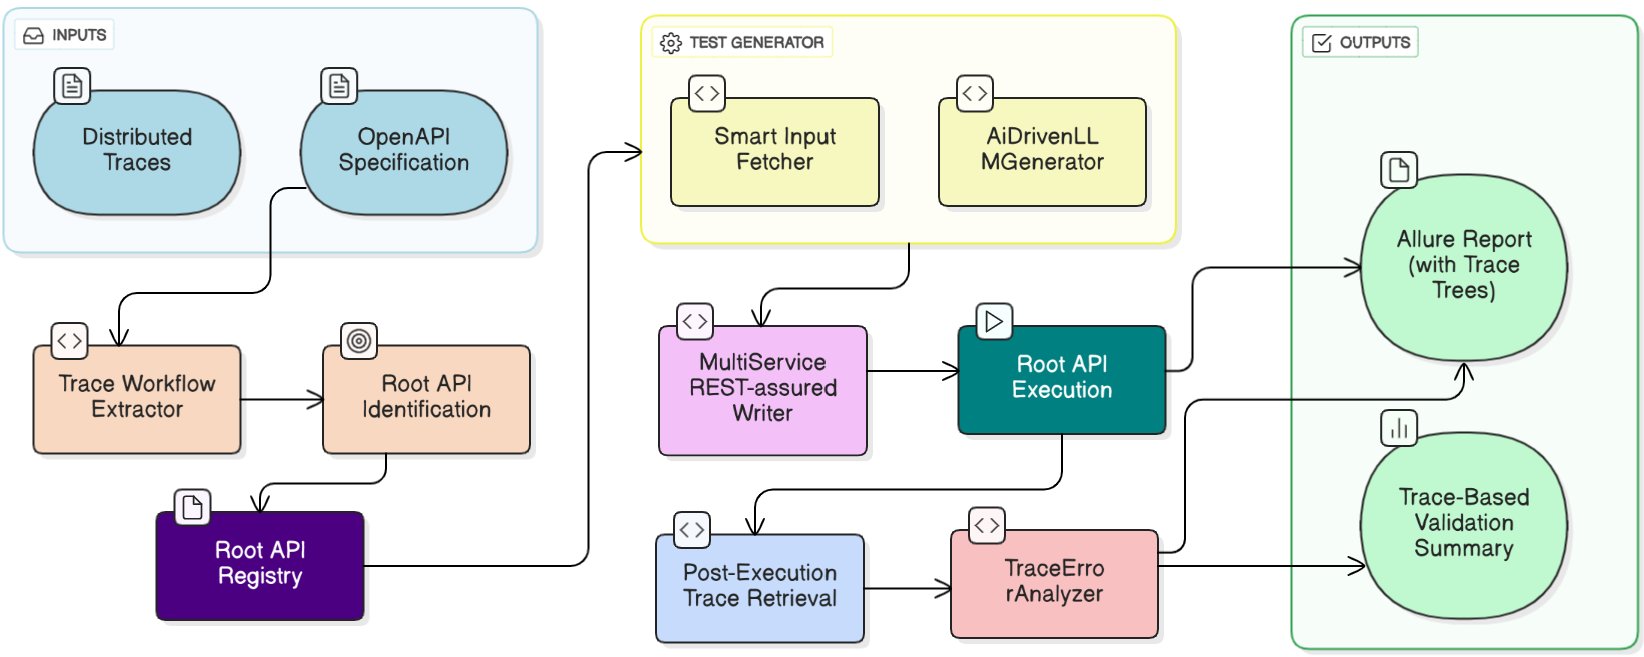
\includegraphics[width=\textwidth]{figs/Res_flow.png}
    \caption{\textsc{MIST}'s trace-driven Root API Mode testing pipeline. Inputs (\textit{blue}) consist of distributed traces and OpenAPI specifications. The processing flow identifies root APIs and maintains a registry (\textit{purple}), then generates tests through Smart Input Fetching and LLM-based synthesis (\textit{yellow}), writing executable cases (\textit{pink}). These are executed against the system (\textit{teal}), followed by trace retrieval, Trace-Shape-Oracle evaluation, and error analysis (\textit{red}). Outputs (\textit{green}) provide Allure reports with trace trees, validation summaries, mined fault-type proposals, and updates to the Root API Registry.}

  \label{fig:dataflow}
\end{figure*}
%====================================================================
\subsection{Tool Architecture}\label{ssec:arch}
\textsc{MIST} is packaged as a Maven multi-module project so that the core contribution can be vendored or evaluated without dragging in any particular host framework.  Four modules compose the tool:
\begin{itemize}[leftmargin=*]
  \item \texttt{mist-core}: the contribution.  It contains the Trace
        Shape Oracle (\texttt{io.mist.core.oracle.shape.*}), the
        Adaptive Fault Taxonomy (\texttt{io.mist.core.fault.*}), the
        Multi-Root Sequence pipeline, the Semantic Dependency Registry,
        and the public test-generation SPI.  By construction, no class
        in \texttt{mist-core} imports the upstream RESTest framework.
  \item \texttt{mist-llm}: a separable LLM client abstraction
        (\texttt{io.mist.llm.LLMClient}) with backends for Ollama,
        Gemini, and OpenAI-compatible HTTP APIs, plus a SHA-256-keyed
        on-disk response cache for reproducibility under
        \texttt{-Drandom.seed}.
  \item \texttt{mist-restest-adapter}: engineering glue that
        implements \texttt{mist-core}'s SPI (OpenAPI loader, test-case
        data model, JUnit/REST-Assured writer) against the upstream
        \textsc{RESTest}~\cite{martin2019restest} scaffolding.
  \item \texttt{mist-cli}: a standalone entry point
        (\texttt{io.mist.cli.MistMain}) shipped as \texttt{mist.jar};
        invoking \texttt{java -jar mist.jar config.properties} runs
        \textsc{MIST} without traversing any RESTest \texttt{main}
        class.  A thin delegation in the legacy RESTest entry point
        preserves the \texttt{java -jar restest.jar} launch path for
        backward compatibility.
\end{itemize}

The pipeline itself comprises eight subsystems; the first six are inherited from the trace-driven generator's earlier life and the last two are this paper's headline contributions.

\begin{enumerate}[leftmargin=*]
  \item \textbf{Trace Workflow Extractor}
        \hfill(\S\ref{ssec:extract})\\
        Parses OpenTelemetry~\cite{opentelemetry} or Jaeger~\cite{jaeger2017} span logs to extract complete workflow scenarios
        and identify root API endpoints that serve as natural system entry points (Algorithm~\ref{alg:extract}).
  \item \textbf{Test Generator}
        \hfill(\S\ref{ssec:gen})\\
        Generates test cases in two modes: (i)~\emph{Root API Mode}---single entry-point calls with
        trace-based post-execution validation; and (ii)~\emph{Multi-Step Replay}---ordered inter-service
        steps with dependency-aware execution; both using LLM-driven parameter synthesis and
        smart input fetching for realistic test data (Algorithm~\ref{alg:generate}).
  \item \textbf{Multi-Service Test Writer}\\
        Emits JUnit/REST-Assured test classes for both modes with
        integrated trace collection and comprehensive Allure reporting.
  \item \textbf{Trace-Aware Execution Engine}\\
        Executes tests (entry-point or multi-step) and captures trace identifiers.  Integrates a short enhancement loop for failed cases: the loop fixes inputs and re-executes in rounds, preserving reporting and analysis.
  \item \textbf{AI-Powered Trace Analysis Engine}\\
        Fetches execution traces, performs hierarchical failure analysis using
        \textit{TraceErrorAnalyzer}, and provides LLM-driven root-cause diagnosis
        for the complete microservice interaction chains triggered by test executions.
  \item \textbf{Root API Registry System}
        \hfill(\S\ref{ssec:registry})\\
        Maintains a persistent catalog of discovered root APIs with their complete
        microservice interaction patterns, enabling long-term architectural analysis
        and auditability.  The registry is observational: generator-side scenario
        deduplication is performed later by the Test Generator, not by the registry.
  \item \textbf{Trace Shape Oracle}~(new)
        \hfill(\S\ref{ssec:tso})\\
        A learner-oracle pair that ingests a small seed corpus of
        known-good traces and produces four families of per-API
        invariants---span-tree shape, status propagation, timing
        envelope, and response envelope---then checks each subsequent
        live trace against them at first-class assertion strength.
  \item \textbf{Adaptive Fault Taxonomy}~(new)
        \hfill(\S\ref{ssec:adaptfault})\\
        A typed registry of \texttt{FaultType} records, populated from
        a default YAML and extended at runtime by a
        \texttt{FaultMiner} that prompts an LLM with OpenAPI parameter
        descriptions and observed 4xx/5xx responses.  Each
        \texttt{FaultType} carries its own applicability matrix
        (OpenAPI types, parameter locations) so the Sniper Strategy
        automatically gates mined faults to the parameters they make
        sense for.
\end{enumerate}




\noindent%
Figure~\ref{fig:dataflow} depicts the complete trace-driven testing pipeline, from initial trace extraction to AI-powered failure analysis. The diagram demonstrates the transformation of multi-service traces into focused single-API tests, ensuring comprehensive validation through post-execution trace analysis. Details regarding mode-specific generation and execution are provided in Section~\ref{ssec:gen-modes}.

%--------------------------------------------------------------------
\subsection{Trace-Driven Root API Extraction}
\label{ssec:extract}
\begin{algorithm}[tb]
\caption{TRACE\_WORKFLOW\_EXTRACTOR}\label{alg:extract}
\footnotesize
\begin{algorithmic}[1]
\Require\;{Path to trace file or directory}
\Ensure\;{List of \textsc{WorkflowScenario}s}
\State Parse JSON/JSONL files into span objects
\State $spansByTrace \gets$ Group spans by \texttt{traceId}
\ForAll{$(traceId, spans) \in spansByTrace$}
    \State $scenario \gets$ new \textsc{WorkflowScenario}
    \State $stepIndex \gets \{\}$ \Comment{spanId → WorkflowStep mapping}
    \ForAll{$span \in spans$}
        \State $step \gets$ \textproc{CreateWorkflowStep}$(span)$
        \State Extract HTTP method, path, headers, body from span tags
        \State Extract timing and status information
        \State \textproc{ExtractFieldsFromUrl}$(step,\;\texttt{http.target}\;\text{or}\;\texttt{http.url})$ \Comment{Regex-map UUID/long-int/noun-prefixed segments to typed keys; populate \texttt{inputFields} only — URL path values are client-supplied inputs, not produced outputs}
        \State $stepIndex[span.spanId] \gets step$
    \EndFor
    \State Link parent-child relationships using span references
    \State Identify root steps (spans with no parents)
    \State Add root steps to $scenario$
    \State Add $scenario$ to results
\EndFor
\State \textproc{MergeScenariosByDataDependency}$(scenarios)$
\Comment{Phase~1: temporal guard; ignore HTTP-meta keys; record \texttt{dataProvenance};
         promote merged consumer to top-level root (\S\ref{ssec:multiroot})}
\State \textproc{MergeScenariosBySessionTimeWindow}$(scenarios,\;\Delta_{\max},\;R_{\max})$
\Comment{Phase~2: group by \texttt{sessionIdentifier} (client IP); sort by \texttt{startTimeMicros};
         sliding-window merge when gap $<\!\Delta_{\max}$ and root count $<\!R_{\max}$ (\S\ref{ssec:multiroot})}
\State \Return scenarios
\end{algorithmic}
\end{algorithm}

\paragraph{URL Path Parameter Extraction.}
Production OpenTelemetry traces often lack \texttt{http.request.body} and \texttt{http.response.body} tags because many instrumentation frameworks omit payload capture for performance reasons. To recover business-critical identifiers in this setting, we implement \textproc{ExtractFieldsFromUrl}, which analyses the \texttt{http.target} (or \texttt{http.url}) tag of every span using two regular expressions: (i) a UUID pattern \verb|[0-9a-fA-F]{8}(-[0-9a-fA-F]{4}){3}-[0-9a-fA-F]{12}| and (ii) a long-integer pattern \verb|\d{5,}|. When a match is found, the immediately preceding path segment is used as a semantic key prefix; for example, the path \texttt{/api/v1/accounts/AAA-BBB} yields \texttt{accountId = AAA-BBB}, and \texttt{/api/v1/order/12345/pay} yields \texttt{orderId = 12345}. A curated noun-to-key table covers the most common REST resource nouns observed in the TrainTicket system (\texttt{order}, \texttt{trip}, \texttt{account}, \texttt{route}, \texttt{train}, \textit{etc.}); any unrecognised noun falls back to a stable hash-based key \texttt{pathId\_\{hash\}} to ensure consistent matching across traces. Extracted values are stored exclusively in \texttt{inputFields} of the \textsc{WorkflowStep}: URL path parameters are client-supplied identifiers that \emph{select} a resource; they are not values \emph{produced} by the API call itself. Storing them in \texttt{outputFields} would cause the cross-trace dependency merger to treat any two API calls that reference the same path segment as causally linked, creating false-positive merges among unrelated traces.

\paragraph{Cross-Trace Data Dependency Merging and Provenance.}
After all per-trace scenarios are built, \textproc{MergeScenariosByDataDependency} runs a fixed-point loop to link independent traces into composite workflows. For each pair of scenarios $A$ and $B$ the algorithm iterates over the Cartesian product of their extracted field maps seeking matching key–value pairs. Three correctness guards filter spurious matches: (i) a \emph{temporal guard} requiring \(\textit{producerEnd} < \textit{consumerStart}\) so that only causally plausible orderings are merged; (ii) an \emph{ignore set} that suppresses generic HTTP metadata keys (\texttt{http.method}, \texttt{http.url}, \texttt{http.target}, \texttt{http.path}, \texttt{http.request.body}, \texttt{http.response.body}) that would cause false positive links; and (iii) \emph{provenance recording}—on a successful merge, the consumer step's \texttt{dataProvenance} map is annotated with the exact key–value pair that justified the merge (e.g., \texttt{accountId $\to$ AAA-BBB}). This annotation propagates the causal evidence downstream to the test generator, enabling it to guarantee that the merged step receives the precise ID from its proven producer rather than an overwritten or colliding value from the shared runtime context.

%--------------------------------------------------------------------
\subsection{Multi-Root Sequence Model}
\label{ssec:multiroot}

A critical design decision governs how a merged consumer scenario is incorporated into the producer scenario. A naive approach would attach the consumer's root step as a \emph{child} of the matching producer step, yielding a deeper tree. This is incorrect: the consumer root API is an independent, externally invoked entry point (e.g., \texttt{POST /api/v1/orders}) and must be executed as a separate top-level call in the test suite—not as an internal sub-span.

Our system implements the \emph{Multi-Root Sequence model}: on a successful merge, the \textproc{MergeWith} method \emph{promotes} the consumer root step to a new top-level root within the producer's \textsc{WorkflowScenario}. Two metadata fields are set on the promoted step: \texttt{mergedRoot = true} and \texttt{producerRootIndex}, which records the 1-based local position of the earliest preceding root inside the same component that actually produces data consumed by this root (looked up via the reverse-adjacency set built during Weakly Connected Component analysis). This correctly handles fan-out topologies in which a single producer root serves multiple downstream consumers---a naive ``previous list position'' heuristic would wrongly record the most recent sibling as the producer. The result is a single \textsc{WorkflowScenario} whose \texttt{rootSteps} list contains multiple independent Root APIs in causal order, e.g., \textit{Root~1: POST /api/v1/trips}, followed by \textit{Root~2: POST /api/v1/orders} (which depends on the \texttt{tripId} produced by Root~1).

\paragraph{Five-phase end-to-end scenario pipeline.}
The full scenario-processing pipeline now spans both extraction and generation. The extractor performs Phase~1 and Phase~2; the generator then performs Phase~2.5, Phase~3, and Phase~4 before variant generation begins.

\emph{Phase~1---Value-based merging.} \textproc{MergeScenariosByDataDependency} executes a fixed-point loop (as described above) to link traces that share matching business-data values. This phase is highly precise—it only merges when a concrete key–value pair is shared between a producer and a consumer—but it requires that those values appear in the raw span attributes. In practice, many production OpenTelemetry deployments omit \texttt{http.response.body} and \texttt{http.request.body} for performance reasons, leaving Phase~1 unable to recover dynamically-generated identifiers (e.g., a freshly-created order ID).

\emph{Phase~2---Session-based heuristic merging.} \textproc{MergeScenariosBySessionTimeWindow} handles the common case where response bodies are absent. Each \textsc{WorkflowScenario} is extended with three metadata fields: \texttt{sessionIdentifier} (extracted from the \texttt{http.client\_ip} span tag, falling back to \texttt{UNKNOWN\_SESSION}), \texttt{startTimeMicros} (the minimum span start time in the trace), and \texttt{endTimeMicros} (the maximum of $\text{startTime} + \text{duration}$ across all spans—computed because Jaeger traces record \texttt{duration} but not \texttt{endTime} directly). The algorithm groups scenarios by \texttt{sessionIdentifier}, sorts them chronologically within each group, and applies a sliding-window merge: if the next scenario starts after the current accumulator ends, and the gap is less than a configurable threshold $\Delta_{\max}$ (default 60 s), and the accumulator has fewer than $R_{\max}$ roots (default 10), the next scenario is appended via \texttt{appendSequentialScenario}. This method transfers all \texttt{rootSteps} from the absorbed scenario, marks each transferred root with \texttt{mergedRoot=true} and a sequential \texttt{producerRootIndex}, and extends \texttt{endTimeMicros}. Absorbed scenarios are removed from the master list.

When \texttt{sessionIdentifier == UNKNOWN\_SESSION} (traces whose \texttt{http.client\_ip} tag was not captured by the instrumentation framework), the algorithm applies a \emph{conservative fallback} rather than skipping the bucket entirely: a reduced gap threshold (default 15~s) and a reduced root cap (default 3 roots), both capped below the configured $\Delta_{\max}$ and $R_{\max}$ respectively. This preserves multi-root assembly for legitimately related traces whose client-IP metadata was dropped by the observability pipeline while preventing wild merges across unrelated requests that only share the absence of session metadata.

On the \emph{traces-1772605095842.json} workload (154 isolated single-root scenarios), Phase~2 reduced the scenario count to 15--20 Multi-Root Sequential Scenarios, each representing a coherent user session such as \emph{Login $\to$ Search $\to$ Select Trip $\to$ Create Order $\to$ Pay}.

\emph{Phase~2.5---Global single-root deduplication.}
After trace extraction but before shared-pool generation, the Test Generator performs a global filter over the incoming scenario list.  It keeps only the \emph{first} standalone 1-root scenario per normalized API key (e.g., \texttt{GET\_\_api\_v1\_adminbasicservice\_adminbasic\_stations}) and discards later duplicates.  Multi-root scenarios are preserved unchanged because they may differ in downstream structure even when they share a root API.  This phase addresses \emph{trace amplification}: repeated page loads or repeated button clicks may produce many identical 1-root traces that would otherwise each become their own \texttt{Flow\_Scenario\_N.java} file.  The implementation maintains a shared \texttt{seenSingleRootApis} set that is also reused by Phase~4 below.

\emph{Phase~3---Scenario Shattering (connected-component partitioning).}
Phase~2's temporal heuristic can over-merge: it may group API calls that share a session window but have no semantic data dependency (e.g., interleaved requests from multiple browser tabs, or an unrelated health-check adjacent to a user action). Testing an isolated API inside a fat sequential test case is an anti-pattern---a failure in an independent step masks execution of subsequent dependent steps, producing flaky tests and obscuring real faults.

The \textsc{ScenarioOptimizer} post-processes every multi-root scenario ($|\texttt{rootSteps}| > 1$) before variant generation. For each scenario it: (i)~builds a \emph{directed dependency graph} where nodes are the root steps and an edge from node~$i$ to node~$j$ ($j>i$) exists iff \textproc{HasDirectedDependency}$(root_j,\;root_i)$ returns true (consulting the Semantic Dependency Registry to check whether any parameter of the consumer can be satisfied by the producer); (ii)~computes \emph{Weakly Connected Components} via Union-Find with path compression; and (iii)~\emph{shatters} the original scenario into one new \textsc{WorkflowScenario} per component, preserving the chronological order of steps within each partition and reassigning \texttt{mergedRoot}/\texttt{producerRootIndex} metadata. Isolated root steps (those with no incoming or outgoing dependency edges) are decoupled into independent 1-root scenarios that are tested individually, eliminating cross-contamination from unrelated failures.

\emph{Phase~4---Trace decomposition with shared dedup state.}
After shattering, the generator optionally decomposes each remaining multi-root scenario into standalone 1-root baseline scenarios (\texttt{Flow\_Scenario\_N\_RT1}, \textit{etc.}) to guarantee direct per-API coverage.  However, decomposition now consults the same \texttt{seenSingleRootApis} state used in Phase~2.5.  Consequently, if a standalone 1-root scenario for API~$A$ already survived the global deduplication pass, the decomposer will \emph{not} emit an additional \texttt{\_RT} baseline for $A$.  This unifies standalone-scenario deduplication and decomposition-time deduplication in a single consistency mechanism.

\paragraph{Hierarchical naming.}
The test generator traverses the \texttt{rootSteps} list and assigns each root a hierarchical identifier: Root~1 receives prefix \texttt{R1}, Root~2 receives \texttt{R2}, and their respective internal child spans receive prefixes \texttt{R1.1}, \texttt{R1.2}, \texttt{R2.1}, and so forth. In Root API Mode, only the top-level root steps (those marked \texttt{topLevelRoot = true}) are retained in the generated test case; internal spans are pruned because they will be validated through post-execution trace analysis. This distinction preserves merged root APIs while eliminating ordinary internal sub-spans.

\paragraph{Flow-centric test naming.}
Because a single \textsc{MultiServiceTestCase} may now span multiple root APIs from different services, the legacy naming convention—which derived class and method names from the first API's HTTP method and path—is replaced with a flow-centric convention that is invariant to which particular APIs appear in the sequence:

\begin{itemize}[leftmargin=*]
  \item \textbf{Test class:} \texttt{Flow\_Scenario\_}$N$ (e.g., \texttt{Flow\_Scenario\_12}), where $N$ is the scenario counter.
  \item \textbf{Positive variant:} \texttt{test\_positive\_flow\_S}$N$\texttt{\_v}$V$, where $V$ is the variant index.
  \item \textbf{Negative variant:} \texttt{test\_negative\_flow\_S}$N$\texttt{\_v}$V$\texttt{\_fault\_Root}$R$\texttt{\_}$\mathit{TYPE}$, where $R$ is the 1-based index of the targeted root API and $\mathit{TYPE}$ is the \texttt{InvalidInputType} name (e.g., \texttt{OVERFLOW}, \texttt{BOUNDARY\_VIOLATION}).
\end{itemize}

When a negative variant is demoted to positive due to pool exhaustion, both the \texttt{targetFaultRootId} and \texttt{faultTypeCategory} fields are cleared and the method name is rewritten to the positive convention.

\paragraph{Dependency preservation.}
The test writer checks whether a step carries \texttt{mergedRoot = true}. If so, it emits a \texttt{DATA\_DEPENDENCY} edge in the Allure step metadata linking Root~$R$ to its producer Root~$R-1$, and attaches a \textit{Cross-Trace Provenance} attachment listing the inherited key–value bindings. The \texttt{setStepDependencies} method short-circuits the generic \texttt{analyzeDependencies} routine for merged roots to prevent the explicitly set \texttt{DATA\_DEPENDENCY} classification from being overwritten to \texttt{INDEPENDENT}.

\paragraph{Root API Identification and Accessibility Rationale.}
The \textproc{FindFirstBusinessAPI} function identifies the entry-point API call by filtering out authentication spans and selecting the first HTTP operation that represents actual business logic. This trace-driven approach addresses a fundamental challenge in microservice testing: \emph{API discoverability and accessibility}.

In microservice architectures, not all endpoints defined in OpenAPI specifications are directly accessible for testing. Many services implement \emph{internal} or \emph{private} APIs that are only accessible within the service mesh or cluster network, while others require complex authentication workflows or service-to-service communication protocols~\cite{waseem2020testing, zhou2018microservice}. A systematic review of microservice testing challenges identifies API visibility and service discoverability as primary obstacles to effective testing~\cite{microservice-testing-review-2023}.

By extracting root APIs from actual execution traces, we automatically identify the \emph{publicly accessible entry points} that real clients use to interact with the system. This approach ensures that our tests target APIs that are:
\begin{itemize}[leftmargin=*]
\item Actually accessible from external clients
\item Properly authenticated and authorized
\item Integrated with the system's API gateway or service mesh
\item Representative of real-world usage patterns
\end{itemize}

This methodology aligns with established best practices in microservice testing that emphasize focusing on externally accessible interfaces rather than attempting to test all internal service endpoints directly.

\paragraph{Trace Context Preservation.}
Although only the root API is used for test generation, the complete trace context is preserved to enable post-execution validation. This includes the full service interaction hierarchy, expected response patterns, and inter-service dependencies observed in the original execution.

%--------------------------------------------------------------------
\subsection{Test Generation}
\label{ssec:gen}

\subsubsection*{Generation Modes (summary)}\label{ssec:gen-modes}
Modes are introduced in Section~\ref{sec:overview}. Here we summarize their impact on generation only: Root API Mode produces single-call tests anchored at entry points with post-execution trace validation (see Section~\ref{ssec:exec}); Multi-Step Replay emits ordered step sequences with dependency-aware execution for environments that preserve cross-call prerequisites.

\begin{algorithm}[tb]
\caption{TEST\_GENERATOR}
\label{alg:generate}
\footnotesize
\begin{algorithmic}[1]
\Require\;{List of \textsc{WorkflowScenario}s, configured variant count $V_\mathrm{cfg}$}
\Ensure\;{Collection of \textsc{MultiServiceTestCase}s, flow-centric naming}
\State \textproc{DeduplicateSingleRootScenarios}$(scenarios)$
\Comment{Phase~2.5: keep first standalone 1-root scenario per normalized API key; preserve all multi-root scenarios}
\State Group scenarios by entry-point root APIs; build shared parameter pools per group
\State \textproc{ScenarioOptimizer.Shatter}$(scenarios)$
\Comment{Phase~3: connected-component partitioning of fat multi-root scenarios}
\State \textproc{DecomposeMultiRootScenarios}$(scenarios)$
\Comment{Phase~4: emit missing standalone 1-root baselines only if not already covered in Phase~2.5}
\ForAll{$root \in$ all root APIs across all scenarios}
    \State Build \textsc{InvalidInputPool} per parameter of $root$, keyed by $root$'s verb\_path \Comment{Pools cover all roots in Multi-Root Sequences, not only the first}
\EndFor
\State $testCases \gets \{\}$
\ForAll{$scenario \in scenarios$}
    \State $Q \gets$ \textproc{BuildFaultInjectionQueue}$(scenario)$ \Comment{Exhaustive, priority-ordered \textsc{FaultTarget} list (\S\ref{ssec:negtest})}
    \State $V_{\mathit{pos}} \gets \max(1,\;\lceil V_\mathrm{cfg}(1-\rho)\rceil)$;\quad $V_{\mathit{neg}} \gets \max(\lfloor V_\mathrm{cfg}\rho\rfloor,\;|Q|)$
    \State $V \gets V_{\mathit{pos}} + V_{\mathit{neg}}$ \Comment{Dynamic Variant Sizing: override if $V > V_\mathrm{cfg}$}
    \For{$v \gets 1$ to $V$}
        \State $tc \gets$ new \textsc{MultiServiceTestCase}(\textit{flow-centric name})
        \If{$v \leq V_{\mathit{pos}}$}
            \State $isFaulty \gets \mathbf{false}$;\quad $target \gets \emptyset$
        \Else
            \State $isFaulty \gets \mathbf{true}$;\quad $target \gets Q.\text{dequeue}()$ \Comment{\textsc{FaultTarget} = (rootIndex, paramName, type)}
            \State Set $tc.\mathtt{targetFaultRootId} \gets \text{"Root~"}+target.\mathit{rootIndex}$
            \State Set $tc.\mathtt{faultTypeCategory} \gets target.\mathit{type}.\mathbf{name}()$
        \EndIf
        \State $context \gets \{\}$
        \ForAll{$rootStep_i \in scenario.\mathtt{rootSteps}$} \Comment{Traverse all roots in causal order}
            \State $\mathit{faultThis} \gets isFaulty \;\wedge\; (i = target.\mathit{rootIndex})$
            \State \textproc{TraverseStep}$(rootStep_i,\; tc,\; context,\; \text{"R"}i,\; \mathit{faultThis},\; target)$
            \Comment{Non-targeted roots receive strictly valid inputs (Sniper Strategy)}
        \EndFor
        \State Remove steps where $\neg\;\mathtt{isTopLevelRoot}$ \Comment{Prune internal spans; keep all merged Root APIs}
        \If{$isFaulty$ \textbf{and} no valid invalid value was injected}
            \State Demote $tc$ to positive; clear fault metadata
        \EndIf
        \State $testCases \gets testCases \cup \{tc\}$
    \EndFor
\EndFor
\State \Return $testCases$
\end{algorithmic}
\end{algorithm}

\paragraph{Hybrid parameter generation.}
\textproc{TraverseStep} applies a layered strategy that prioritises exactness and realism before diversity:
\begin{itemize}[leftmargin=*]
  \item \textbf{Provenance-first (Priority~0).}  Before consulting any external source, the generator checks the current \textsc{WorkflowStep}'s \texttt{dataProvenance} map. If the required parameter was the key that caused a Phase~1 cross-trace merge, its exact value is used directly. This guarantees that a consumer step receives the precise ID from its proven producer and prevents context collisions when multiple merged traces contribute the same key name.
  \item \textbf{JIT Schema Binding (Priority~0b).}  For scenarios assembled by Phase~2 (session heuristic), no \texttt{dataProvenance} values exist because the merge was temporal, not value-based. The generator therefore applies \emph{Just-In-Time (JIT) Dependency Binding}: for every Root~$N$ step ($N > 1$), it queries the \emph{Semantic Dependency Registry} (described below) to discover which earlier root API likely produces the required parameter. If a match is found, a \texttt{ParamDependency} is added to the \textsc{StepCall}, and the writer emits \texttt{capturedOutputs.get($k$)} code that resolves the value at test runtime from the actual response of Root~$k$. If no prior producer is present in the sequence (the C$\to$B edge case), the generator logs a debug message and falls back gracefully to the standard priority chain below.
  \item \textbf{Trace-derived context (Priority~1).}  Parameters not covered by provenance or JIT binding are resolved from the shared runtime context populated by prior steps' URL-extracted \texttt{inputFields}. This leverages the full set of business identifiers recovered from URL paths without any LLM inference cost.
  \item \textbf{System-resident values (Priority~2).}  \emph{Smart Input Fetching} supplies existing IDs, codes, or tokens (used with configurable probability) to ensure valid baselines when the trace context is insufficient. The fetcher first tries endpoints observed as \emph{proven producers} in the original workflow trace before falling back to the static registry (see Section~\ref{ssec:smartfetch}).
  \item \textbf{LLM-based synthesis (Priority~3).}  \emph{AiDrivenLLMGenerator} proposes semantically diverse candidates when all higher-priority sources are exhausted or unavailable. The prompt is \emph{schema-complete}: it includes the endpoint (method + path), parameter name and location, type and format, description, example, required/optional status, and all available OpenAPI constraints (enums, numeric bounds, length limits, and regex patterns).
\end{itemize}

\paragraph{Schema-complete prompt construction.}
Positive-value generation uses a strict LLM persona specialized for API test-data synthesis. For each parameter, the generator constructs a structured prompt with four sections: \emph{API Context}, \emph{Parameter Details}, \emph{Constraints}, and \emph{Instructions}. The instruction block explicitly requires the model to return \emph{exactly} $N$ values, forbids markdown or explanatory text, and mandates compliance with the declared type, format, and constraints. When an enum is present, the prompt states that the model must choose \emph{only} from the allowed-value list. This design reduces hallucinated types (e.g., strings for integer enums) and improves adherence to OpenAPI semantics while preserving domain realism.

\paragraph{Dynamic shared pools and uniqueness.}
Shared parameter pools are sized dynamically from the configured variant count and the arity of the root API, rather than being capped by a fixed semantic-expansion budget. Values harvested from Smart Input Fetching and the LLM are merged into a uniqueness-preserving set before being stored in \texttt{sharedParameterPools}. During positive generation, the first business root draws from these pools via random selection instead of deterministic modulo rotation, greatly reducing clone variants. To prevent residual collisions, generated positive payloads are fingerprinted and retried several times; only globally unique payloads are admitted to the final test suite.

\paragraph{Semantic Dependency Registry.}
To support Priority~0b JIT binding, we introduce the \emph{Semantic Dependency Registry}, a lightweight dictionary built at startup from the loaded test configurations and per-service OpenAPI specifications. Producers are registered by three rules: a \emph{strong} rule for POST/PUT on entity resources (the trailing noun yields the entity's ID stem); an \emph{authentication} rule for POST endpoints whose tail is \texttt{login}, \texttt{authenticate}, or \texttt{signin}, which return session identifiers; and a \emph{weak} rule (restricted to POST/PUT, since GET/DELETE consume or destroy rather than emit IDs) that treats an ID-like path parameter as evidence of producing that ID. Consumer parameters are recognised by two complementary patterns: an \emph{ID-suffix} form (e.g.\ \texttt{orderId}, \texttt{account\_id}) and an \emph{ID-prefix} form (e.g.\ \texttt{id\_account}, \texttt{idAccount}), the latter requiring an explicit separator after the prefix to avoid false positives on English words such as \texttt{identity} or \texttt{idle}. Generic \texttt{\{id\}}/\texttt{\{uuid\}} path parameters inherit their stem from the preceding path segment. Each recognised consumer parameter is bound to a producer by a multi-axis scorer with fixed weights over rule strength, HTTP method, service-name affinity to the stem, and a cross-service bonus. At generation time, \textproc{FindProducer} returns every candidate for the parameter's stem; the generator wires the nearest preceding root whose canonicalised key matches one, ensuring each heuristic recommendation is grounded in the actual scenario topology.

\paragraph{Variants and efficiency.}
To balance coverage with cost, variants follow a consistent policy:
\begin{enumerate}[leftmargin=*]
  \item \textbf{High-fidelity baseline:} start from fetched/trace-seeded values to exercise realistic success paths.
  \item \textbf{Boundary exploration:} perturb constraints (ranges, enums, required/optional fields) to expose robustness issues.
  \item \textbf{Schema-aware semantic diversity:} use LLM-generated values to probe alternative but plausible interpretations while still respecting endpoint context and OpenAPI constraints.
  \item \textbf{Targeted negatives:} apply the Sniper Strategy (Section~\ref{ssec:negtest}) to inject exactly one fault per variant into exactly one root API while preserving valid inputs for all other roots.
\end{enumerate}

\paragraph{Context preservation.}
During generation, we maintain a runtime context for potential data dependencies and reuse across parameters; during execution, we anchor the call at the entry point and defer inter-service validation to post-execution trace analysis. This separation keeps execution authentic while enabling deep, trace-based oracles without replaying downstream steps for interservice communication.



\subsection{Test Case Types}\label{ssec:test-types}
The generator produces two case families with compact, configuration-driven oracles and AI support. \emph{Positive} cases exercise valid inputs and expect success; \emph{Negative} cases intentionally introduce invalid or semantically inconsistent inputs and expect errors.

\begin{table}[t]
\centering
\caption{Test Types and Validation Rules}
\label{tab:test-types}
\renewcommand{\arraystretch}{1.15}\setlength{\tabcolsep}{4pt}
\begin{tabularx}{\columnwidth}{>{\bfseries}p{0.24\columnwidth} X X}
\toprule
Type & Status-code rule & LLM response rule (2XX only) \\
\midrule
Positive & Pass only if \texttt{actual} $=$ \texttt{expectedStatus} (from configuration) & Fail if analysis reports a soft error; otherwise pass \\
Negative & Pass if the response status is non-2XX (i.e., $\texttt{actual} \notin [200, 300)$) --- the API clearly rejected the invalid input; 2XX proceeds to soft-error check & Pass if analysis reports a soft error; otherwise fail \\
\bottomrule
\end{tabularx}
\end{table}

\paragraph{Negative case generation.}\label{ssec:negtest}
\noindent Negative test generation follows a five-stage pipeline:

\begin{enumerate}[leftmargin=*]
  \item \textbf{Pool construction (all roots).} Per-root-API \textsc{InvalidInputPool} objects are built for \emph{every} root API in a scenario, including all merged root APIs in Multi-Root Sequences—not merely the first business step. Each pool is keyed by the root's \texttt{verb\_path} identifier and stores invalid values grouped by \textsc{InvalidInputType}.

  \item \textbf{Prioritized fault synthesis.} Invalid values are generated by the LLM across eight fault categories. Within each pool, the round-robin cursor traverses these categories in a fixed \emph{high-risk-first} order: \textsc{Boundary\_Violation} $\to$ \textsc{Overflow} $\to$ \textsc{Null\_Input} $\to$ \textsc{Empty\_Input} $\to$ \textsc{Special\_Characters} $\to$ \textsc{Type\_Mismatch} $\to$ \textsc{Regex\_Mismatch} $\to$ \textsc{Semantic\_Mismatch}. This ordering ensures that the highest-risk edge cases---boundary violations and overflows, which are the most likely to reveal unguarded server-side validation gaps---are exercised before lower-risk semantic mismatches.

  \item \textbf{Fault injection queue construction.} \textproc{BuildFaultInjectionQueue} enumerates every \textsc{FaultTarget} tuple $(\mathit{rootIndex},\;\mathit{paramName},\;\mathit{type})$ across all roots and all parameters by exhausting each pool's round-robin cursor. The resulting queue length equals the total number of distinct invalid values in the scenario, serving as a lower bound on the number of negative variants required for exhaustive coverage.

  \item \textbf{Dynamic variant sizing.} Let $V_\mathrm{cfg}$ be the configured variant count and $\rho$ the configured faulty ratio. The generator sets the positive base $V_{\mathit{pos}} = \max(1, \lceil V_\mathrm{cfg}(1-\rho)\rceil)$ and the negative count $V_{\mathit{neg}} = \max(\lfloor V_\mathrm{cfg}\rho\rfloor,\;|Q|)$, where $|Q|$ is the fault queue length. The total variant count is $V = V_{\mathit{pos}} + V_{\mathit{neg}}$. When $V > V_\mathrm{cfg}$, the configured count is automatically overridden to guarantee that every \textsc{FaultTarget} in the queue is exercised at least once.

  \item \textbf{Sniper Strategy injection and oracle application.} Each negative variant dequeues exactly one \textsc{FaultTarget} and applies its invalid value to the designated parameter of the designated root API. All other root APIs in the same sequence receive strictly valid, positive inputs, guaranteeing that the workflow executes normally up to the targeted step. This \emph{Sniper Strategy} isolates the fault to a single injection point, preventing cascading failures from masking the true server-side validation behaviour. The target root identity and fault type category are persisted on the \textsc{MultiServiceTestCase} object (\texttt{targetFaultRootId} and \texttt{faultTypeCategory}) and propagated to Allure for structured reporting. If a negative variant fails to obtain an invalid value (e.g., due to pool exhaustion), it is demoted to a positive test and its fault metadata is cleared.
\end{enumerate}

AI is central to both generation and validation: LLMs synthesize semantically inconsistent inputs and detect \emph{soft errors} in successful responses, ensuring negative testing covers business-logic semantics beyond surface constraints.

\paragraph{Configuration.}
Negative test generation is governed by two properties: \texttt{faulty.ratio} controls the proportion of negative variants requested; \texttt{faulty.round-robin} (when \texttt{true}, the default) activates the queue-based Sniper Strategy. When set to \texttt{false}, a random selection mode is used instead: 1--3 parameters are selected at random per test, fault types and values may repeat, and no exhaustiveness guarantee is provided.

\subsection{Root API Registry for Systematic Discovery and Management}\label{ssec:registry}

We introduce a concise \emph{Root API Registry} that persistently catalogues unique entry-point APIs (root APIs) together with their complete microservice interaction trees. The registry is populated automatically from distributed traces and used to reason about dependency changes, audit architectural behavior, and support regression targeting. Importantly, the registry is an \emph{observational artefact}: it records what was seen in traces, but it does not directly gate or filter the generator's scenario list.

\paragraph{Design summary.}
The implementation consists of three lightweight components: (i) \textbf{RootApiRegistry}, a thread-safe manager that deduplicates root APIs and persists the registry; (ii) \textbf{RootApiEntry}, which represents a single root API and stores the set of distinct interaction trees observed for it; and (iii) \textbf{ApiTree}, a normalized tree that captures service call hierarchies (service, method, path) without request payloads. Trees are compared using structure-aware hashing to avoid storing duplicates while allowing multiple valid patterns per root API.

\paragraph{Applications.}
Distributed tracing has been shown to capture end-to-end causal relationships at scale, enabling dependency reconstruction and performance analysis (e.g., \textsc{Dapper}~\cite{sigelman2010dapper} and \textsc{Pivot Tracing}~\cite{mace2015pivot}). Empirical microservice benchmarks demonstrate that a single outward-facing API can exercise \emph{different internal call paths} under varying inputs and workloads, motivating the storage of multiple trees per root API (\textsc{DeathStarBench}~\cite{gan2020deathstarbench}). Systematic studies of microservice testing highlight persistent challenges in API discoverability, dependency awareness, and regression impact analysis, calling for trace-informed and automation-friendly artefacts~\cite{waseem2020testing}. Our registry operationalizes these insights by: (i) enumerating externally exercised entry points; (ii) recording the corresponding interaction trees; and (iii) persisting them for CI-aware test planning and change impact analysis.

\paragraph{Outputs and usage.}
The registry materializes two artefacts: (a) a de-duplicated list of root APIs (HTTP method + normalized path) discovered from traces; and (b) per-root \emph{sets of interaction trees} that document observed service-call hierarchies. The artefacts are stored in JSON for inspection and downstream analysis, and are updated incrementally across runs. Duplicate \emph{test generation} is controlled separately by the generator's Phase~2.5 single-root deduplicator and the shared dedup state reused during Phase~4 decomposition.

%--------------------------------------------------------------------
\subsection{Smart Input Fetching for Parameter Generation}\label{ssec:smartfetch}

The \emph{primary objective} of Smart Input Fetching is to harvest \emph{system-resident inputs} (e.g., existing identifiers, tokens, codes) so that requests use values that truly exist in the deployed environment. This prevents spurious client-side failures (e.g., \texttt{404} for non-existent IDs, \texttt{401} for missing tokens) and strengthens the oracle: we can observe whether an API succeeds or fails \emph{even with correct inputs}. Starting from valid seeds also enables purposeful negative tests by applying controlled mutations or withholding context values. The \emph{secondary objective} is efficiency and diversity: reduce expensive LLM calls while maintaining variety through dynamically sized shared pools and schema-aware prompting.

\paragraph{Mechanism and integration.}
Configuration is supplied via the experiment's properties (a feature toggle, a probability for using fetched values, the location of the registry, cache time-to-live, and the base service URL) and passed to the generator at startup. The generator reads these settings once, constructs a fetching configuration and fetcher, and consults an \emph{input fetch registry} that maps parameter patterns to provider endpoints with JSONPath-based extractors. Optional LLM-assisted discovery proposes new mappings from API metadata and service patterns. A cache bounds network overhead and stabilizes fetched values across a run; authentication hints can be provided for protected providers.


\paragraph{Testing intent and benefits.}
Using system-resident inputs makes tests representative and diagnostic: APIs are exercised under valid preconditions, revealing server-side faults that would be masked by invalid data. From these valid baselines, we construct deliberate negatives by perturbing selected fields, violating constraints, or withholding dependencies. The mechanism remains orthogonal to the test-generation core: fetched values enter the same runtime context used for parameter injection and validation, while caching and timeouts keep cost predictable.


%--------------------------------------------------------------------
\subsection{Trace Shape Oracle}\label{ssec:tso}

\paragraph{Motivation.}
Every component described so far---trace ingestion, Multi-Root Sequence
assembly, hybrid input generation, Sniper Strategy fault injection---is
on the \emph{generation} side of the pipeline.  Its task is to produce
a call that will exercise interesting cross-service behaviour.  The
\emph{oracle} side has historically been thinner: an HTTP status check
plus a soft-error rule cache that detects success-coded 2xx responses
whose body contains a primary-field value outside the learned success
set.  Both checks operate at the boundary of the call under test; the
trace, once captured by \textsc{TraceErrorAnalyzer}, was used for
\emph{diagnosis} of an already-detected failure rather than as a source
of \emph{detection}.  This is a missed opportunity: the trace carries
strictly more information than the response (the full induced span
subtree, every internal status code, every per-span duration), and
every OpenTelemetry-instrumented microservice already emits it.

The Trace Shape Oracle promotes the trace from diagnostic side-channel
to checkable assertion.  A small, off-line \emph{learner} reads a
labelled seed corpus of known-good traces; an on-line \emph{oracle}
consumes the freshly-pulled trace of each test step and produces a
structured verdict against the learned invariants.  Soft-error
detection becomes one of four invariant families rather than a
stand-alone artefact.

\paragraph{Invariant taxonomy.}
The oracle decomposes a per-root-API invariant into four families,
each with a learner and an oracle that share an interface
\texttt{ShapeInvariant} returning a \texttt{TraceShapeVerdict}
$\langle \mathit{passed}, \mathit{violations}, \mathit{evidence} \rangle$.

\begin{description}[leftmargin=0pt,style=nextline]
  \item[\textbf{SpanTreeShapeInvariant.}]  For each root API, the
        learner records the \emph{set} of $(\textit{parent.service},
        \textit{child.service})$ edges that appear in at least
        $K\%$ ($K{=}80$ by default) of known-good traces, together
        with the per-level fan-out distribution.  At evaluation
        time, the oracle flags (i)~edges in the live trace that the
        learned set does not contain (\emph{unexpected downstream
        service call}), (ii)~edges in the learned set that the live
        trace does not contain (\emph{dropped downstream service
        call}), and (iii)~fan-out outliers (a span has three times
        more children than the learned distribution allows).  Set
        semantics, not sequence semantics, are used at each level so
        that the inherently non-deterministic call ordering within a
        microservice does not produce false positives.
  \item[\textbf{StatusPropagationInvariant.}]  Per root API and per
        tree level, the learner records the distribution of
        \texttt{http.status\_code} and \texttt{otel.status\_code}
        seen across known-good traces.  The oracle flags any span
        whose status falls outside the learned distribution at its
        tree position.  This invariant subsumes the existing
        \textsc{TraceErrorAnalyzer} rule that treats
        \texttt{otel.status\_code=ERROR} as a flag, but parameterises
        the rule per root API so that a service whose 4xx is part of
        a normal control-flow path is not flagged as a failure.
  \item[\textbf{TimingEnvelopeInvariant.}]  Per root API, the
        learner records total-duration percentiles
        $(p_{50}, p_{95}, p_{99})$ and per-span percentiles.  The
        oracle flags a trace whose total duration exceeds the
        learned $p_{99}$ or whose individual span exceeds its learned
        $p_{99}$ by a factor of at least~2.  Because timing
        invariants are intrinsically noisy in production microservice
        workloads, this family ships at \texttt{WARNING} severity
        rather than \texttt{ERROR}.
  \item[\textbf{ResponseEnvelopeInvariant.}]  Per root API, the
        learner records the success-set and failure-set of the
        primary status field observed in the response body of
        known-good traces.  The oracle flags a 2xx response whose
        primary field falls outside the success set; if the value
        is in the known failure set it is reported as a hard
        failure; otherwise it is escalated to the LLM classifier
        used by the legacy soft-error rule cache and the verdict is
        added to the appropriate set.  This family is the direct
        successor to \texttt{SoftErrorRuleCache} and preserves its
        on-disk persistence semantics; the rule cache class is
        retired.
\end{description}

\paragraph{Learning algorithm and seed corpus.}
The learner consumes a directory of trace files plus a manifest
\texttt{seed-trace-labels.json} that marks each trace as
\texttt{KNOWN\_GOOD} (default) or \texttt{KNOWN\_BAD}.  For each
distinct $(\textit{method}, \textit{path})$ root-API tuple, the
learner groups all known-good traces and computes the four invariants
above.  Traces marked known-bad are excluded from the per-family
counts.  The learned invariants are serialised to a JSON file
(\texttt{target/mist-shape-invariants.json}) by atomic rename so that
concurrent oracle reads observe consistent versions.  In practice we
target $N \geq 20$ root APIs with at least~10 occurrences each; on the
TrainTicket corpus this is comfortably met by the 154 traces
described in Section~\ref{ssec:multiroot}.

\paragraph{On-line oracle.}
At test time, after the writer executes a step and pulls the
corresponding trace from Jaeger, it invokes the oracle:
\[
  \mathit{verdict} \;=\; \texttt{TraceShapeOracle.evaluate}(\mathit{rootApi}, \mathit{trace}).
\]
The oracle composes the four families with logical conjunction;
\texttt{verdict.passed} is true iff every family passes, and
\texttt{verdict.violations} is the union of family-level violation
lists annotated with the offending span IDs.  Each verdict is
attached to the Allure step as a structured artefact alongside the
existing trace tree.  Negative tests interpret a violation as a
\emph{pass} (the call was supposed to fail), preserving the soft-error
inversion semantics of Table~\ref{tab:test-types}.

\paragraph{Integration with the rest of the pipeline.}
The Trace Shape Oracle slots between the existing trace-capture stage
and the LLM diagnosis stage in Algorithm~\ref{alg:execute}: after
\textproc{FetchJaegerTraces} populates the trace and before
\textproc{TraceErrorAnalyzer.analyze} is invoked, the oracle is run
and its verdict is added to \texttt{stepResults}.  The downstream
diagnosis engine reads the oracle's structured violations to decide
which spans to focus the LLM root-cause prompt on.  Crucially, the
oracle does not depend on the LLM: in the offline learning phase the
LLM is consulted only for the optional \texttt{ResponseEnvelopeInvariant}
escalation, and \texttt{LLMCallCache} ensures that under
\texttt{-Drandom.seed} the entire pipeline is deterministic.

\paragraph{Relation to prior trace-RCA work.}
Trace-RCA tools such as TraceRCA~\cite{li2021tracerca},
MicroHECL~\cite{liu2021microhecl}, and
ImpactTracer~\cite{xie2023impacttracer} rank suspect spans within an
already-failing trace.  The Trace Shape Oracle, by contrast, decides
whether a trace is failing in the first place against a
SUT-specific, per-API specification that is automatically learned
from a labelled seed corpus.  It complements rather than replaces
RCA: its violation list narrows the downstream prompt that the
LLM-based diagnostic engine uses, which makes the engine's job
strictly easier.

%--------------------------------------------------------------------
\subsection{Adaptive Fault Taxonomy}\label{ssec:adaptfault}

\paragraph{Motivation.}
The Sniper Strategy of Section~\ref{ssec:negtest} draws its invalid
values from a closed eight-category enumeration:
\textsc{Type\_Mismatch},
\textsc{Regex\_Mismatch},
\textsc{Semantic\_Mismatch},
\textsc{Overflow},
\textsc{Empty\_Input},
\textsc{Null\_Input},
\textsc{Special\_Characters}, and
\textsc{Boundary\_Violation}.  These categories are deliberately
generic: they apply equally to a payments service, a train-booking
service, and a music streaming service.  Generic categories work, but
they leave the SUT-specific fault space unexplored.  A booking system
has a notion of an \emph{invalid station name} that no overflow or
null check captures; a payments system has a notion of an
\emph{expired promo code} that no regex mismatch expresses.  These
domain faults are precisely the ones that survive long enough to
appear in production incident reports.

The Adaptive Fault Taxonomy replaces the closed enum with a typed
registry of \texttt{FaultType} records, and adds an LLM-assisted
\texttt{FaultMiner} that proposes SUT-specific categories from the
two artefacts the SUT itself exposes: OpenAPI parameter description
text and observed 4xx/5xx response bodies from prior test runs.

\paragraph{FaultType as data, not enum.}
A fault type is no longer a Java enum constant.  It is a record:
\begin{center}\small
\begin{tabular}{@{}l@{}}
\texttt{record FaultType(} \\
\quad\texttt{String id,}              \\
\quad\texttt{String displayName,}     \\
\quad\texttt{Set<OasType> applicableTo,} \\
\quad\texttt{Set<String> applicableLocations,} \\
\quad\texttt{FaultSource source}      \\
\texttt{)}
\end{tabular}
\end{center}
\noindent The \texttt{id} is a stable identifier suitable for Allure
attachments and statistical aggregation.  \texttt{applicableTo}
constrains the fault to a subset of OpenAPI primitive types
(\texttt{string}, \texttt{integer}, \texttt{number},
\texttt{boolean}, \texttt{array}, \texttt{object}); the Sniper
Strategy consults this set when building the
\texttt{InvalidInputPool} and silently drops nonsensical pairings
such as \textsc{Overflow} on \texttt{boolean}.  \texttt{applicableLocations}
constrains the fault by the OpenAPI \texttt{in} value (\texttt{path},
\texttt{query}, \texttt{header}, \texttt{cookie}, \texttt{body}); a
fault category that only makes sense for body fields cannot be
applied to a path segment.  \texttt{source} records whether the
\texttt{FaultType} was loaded from the default YAML
(\texttt{DEFAULT}) or proposed by the miner
(\texttt{MINED}).

\paragraph{FaultTypeRegistry.}
At startup, \texttt{FaultTypeRegistry} loads the default YAML
\texttt{fault-types.default.yaml}, which reproduces the eight
existing categories verbatim with their applicability matrices, and
optionally a per-SUT YAML pointed to by
\texttt{mist.fault.types.path}.  The registry is immutable after
construction except for the miner's atomic add path.  Every
\texttt{InvalidInputPool} stores its values keyed by
\texttt{FaultType.id} rather than by the legacy enum's
\texttt{.name()}; the eight default ids are byte-identical to the
prior enum names so that existing Allure attachments and
reproducibility seeds do not regress.

\paragraph{FaultMiner.}
The miner is gated by \texttt{mist.fault.mining.enabled} (default
\texttt{false} for predictability).  When enabled, it runs after
each generation cycle:

\begin{algorithm}[t]
\caption{FAULT\_MINER}\label{alg:miner}
\footnotesize
\begin{algorithmic}[1]
\Require\;{OpenAPI spec, observed responses from prior run, current \texttt{FaultTypeRegistry}}
\Ensure\;{Set of proposed \texttt{FaultType} records}
\State $proposed \gets \emptyset$
\ForAll{root API $r$ in spec}
  \ForAll{parameter $p$ of $r$ with non-trivial \texttt{description}}
    \State $failures \gets$ subset of observed 4xx/5xx responses for $r$ that mention $p$
    \State $prompt \gets$ \textproc{BuildMinerPrompt}$(r,\;p,\;failures)$
    \State $candidates \gets$ \textproc{LLM}$(prompt)$ \Comment{up to 3 candidates}
    \ForAll{$c \in candidates$}
      \State $\mathit{ft} \gets$ \textproc{ParseFaultType}$(c)$
      \If{$\mathit{ft}$.id not in \texttt{registry} \textbf{and} $\mathit{ft}$.id not in $proposed$}
        \State $proposed \gets proposed \cup \{\mathit{ft}\}$
      \EndIf
    \EndFor
  \EndFor
\EndFor
\State Persist $proposed$ to \texttt{target/mist-mined-fault-types.yaml}
\State \Return $proposed$
\end{algorithmic}
\end{algorithm}

\noindent The prompt has a strict structure: it summarises the
parameter's OpenAPI declaration (type, format, constraints,
description, examples), enumerates the failed responses that
mention the parameter, and asks for up to three SUT-specific fault
categories with explicit \texttt{applicableTo} and
\texttt{applicableLocations} sets.  Candidates are dedup\-licated
against the default registry and against each other; an id length
filter rejects degenerate proposals such as
\textsc{Invalid\_Value}.  Accepted candidates are persisted to a
timestamped YAML that the user can promote into the per-SUT YAML to
make them permanent.  Because the miner shares the LLM call cache
introduced in Section~\ref{ssec:exec}, re-runs under the same
\texttt{-Drandom.seed} produce the same mined set.

\paragraph{Pool integration.}
The \texttt{InvalidInputPool} class is unchanged in its outer-key
shape: a pool is still indexed by the
\texttt{(rootApiKey, PoolKey(name, location))} composite that
disambiguates same-named parameters at different locations.  The
inner fault dimension changes from \texttt{Map<InvalidInputType, ...>}
to \texttt{Map<String, ...>} keyed on \texttt{FaultType.id}.  The
Sniper Strategy's round-robin cursor visits the default types first
in the priority order of Section~\ref{ssec:negtest}, then visits
mined types in the order they were accepted.  A file-format
migration converts pre-Adaptive-Taxonomy v1 pool files to the v2
format on first save.

\paragraph{Applicability matrix in YAML.}
The previously code-resident schema-aware applicability matrix
(\texttt{InvalidInputType.appliesTo(oasType)} switch) is now data:
each \texttt{FaultType} entry in the default YAML declares an
explicit \texttt{applicableTo} list.  Mined types inherit a
permissive default (\texttt{applicableTo: [string, integer]}) unless
the miner's LLM proposal narrows it.  The Sniper Strategy filters
the pool by both the parameter's OpenAPI type and its location at
pool-construction time, so a fault category that only applies to
\texttt{string} body fields is never enqueued against an
\texttt{integer} path segment.

\paragraph{Reporting and reproducibility.}
Allure attachments use \texttt{FaultType.id} verbatim.  The strict
mode flag inherited from configuration validation
(\texttt{mst.config.strict=true}) extends to fault types: an unknown
id in a per-SUT YAML fails the run rather than being silently
ignored.  The mined YAML is timestamped and seedable; in our
TrainTicket runs the miner consistently proposes domain-specific
categories such as \textsc{Invalid\_Station\_Name},
\textsc{Negative\_Train\_Number}, and
\textsc{Past\_Departure\_Date} that the static eight-category
taxonomy would never produce.

%--------------------------------------------------------------------
\subsection{Trace-Driven Test Execution and Post-Execution Analysis}
\label{ssec:exec}

The execution engine follows the standard lifecycle of test generation, writing, compilation, execution, and reporting. Tests are produced with integrated tracing and reporting hooks suitable for both Root API Mode and Multi-Step Replay. Algorithm~\ref{alg:execute} outlines the overall control flow, and Tables~\ref{tab:exec-overview}--\ref{tab:reporting-artefacts} summarize the execution pipeline, trace retrieval strategies, analysis modes, and reporting artefacts.

\begin{algorithm}[tb]
\caption{GENERATED\_TEST\_EXECUTION\_FLOW}\label{alg:execute}
\footnotesize
\begin{algorithmic}[1]
\Require\;{Generated JUnit test class with multiple test methods}
\Ensure\;{Allure reports with trace analysis}
\State Setup RestAssured with base URI and Allure filters
\ForAll{test method in generated class}
    \State Execute login step to obtain JWT token
    \State $stepResults \gets \{\}$, $failedSteps \gets 0$
    \ForAll{business step $s$ in test method}
        \State Start Allure step with metadata
        \State $startTime \gets$ current microseconds
        \State Build HTTP request with parameters and JWT
        \State $response \gets$ execute HTTP call
        \If{response status matches expected}
            \State $stepResults[s] \gets true$
            \State Attach response to Allure report
        \Else
            \State $stepResults[s] \gets false$, $failedSteps++$
            \State Attach detailed error information
        \EndIf
        \If{response status is 2XX \textbf{and} soft-error validation enabled}
            \State $vr \gets$ \textproc{LLMResponseValidator.validate}(service, endpoint, status, body)
            \State Attach \emph{INTELLIGENT ANALYSIS (Based on Response)} with RCA
            \State Update $stepResults[s]$ according to test type (positive expects SUCCESS; negative expects FAILED)
            \If{verdict changes from pass to fail}
                \State $failedSteps++$
            \EndIf
        \EndIf
        \State $traces \gets$ \textproc{FetchJaegerTraces}$(service, method, path, startTime)$
        \If{traces found}
            \State $analysis \gets$ \textproc{TraceErrorAnalyzer.analyze}$(traces)$
            \State Generate hierarchical trace visualization
            \State Attach trace tree and analysis to Allure
            \If{$analysis.hasErrors()$}
                \State $llmDiagnosis \gets$ \textproc{LLMRootCauseAnalysis}$(analysis)$
                \State Attach AI-generated failure diagnosis
            \EndIf
        \EndIf
        \State Stop Allure step
    \EndFor
    \State Generate comprehensive test summary
    \If{$failedSteps > 0$ OR login failed}
        \State Mark test as FAILED with detailed breakdown
    \Else
        \State Mark test as PASSED
    \EndIf
\EndFor
\end{algorithmic}
\end{algorithm}

\paragraph{Soft-error detection (2XX).}
Soft errors denote business-logic failures surfaced in the response body despite successful HTTP statuses. When enabled, the validator inspects explicit failure flags (e.g., \texttt{status:0}, \texttt{success:false}), error fields (\texttt{error}, \texttt{msg}, \texttt{message}), null or empty \texttt{data} when payloads are expected, and constraint/validation messages. The validator is implemented with large language models that reason over JSON responses to detect \emph{semantic} failures beyond status codes and schemas: it interprets business indicators and messages (including varied phrasing/locales), checks payload consistency (e.g., expected \texttt{data} present and non-empty), and recognises domain-level invariants and constraint violations. Prompts emphasise precision to avoid false positives; evaluation is limited to 2XX responses and produces a concise RCA attached to the report. Positive tests fail when a soft error is detected; negative tests pass when a soft error is detected in a 2XX response.

\paragraph{Execution Overview.}
To facilitate interpretation, Table~\ref{tab:exec-overview} presents the principal execution stages together with their inputs and outputs. Trace acquisition policies are consolidated in Table~\ref{tab:trace-retrieval}. Diagnostic capabilities are organized in Table~\ref{tab:analysis-modes}. Finally, Table~\ref{tab:reporting-artefacts} enumerates the reporting artefacts made available to developers and analysts.

\begin{table*}[t]
\centering
\caption{Execution Pipeline Overview}
\label{tab:exec-overview}
\renewcommand{\arraystretch}{1.15}\setlength{\tabcolsep}{6pt}
\begin{tabularx}{\textwidth}{>{\bfseries}p{0.17\textwidth} X p{0.26\textwidth}}
\toprule
Phase & Key Actions & Outputs \\
\midrule
Setup & Configure RestAssured; register Allure filters; initialize runtime context. & Base URI configured; request/response interceptors active. \\
Authentication & Obtain JWT/token as Step~0 when required; cache for subsequent calls. & Valid auth headers for requests. \\
Step Execution & Build requests with synthesized parameters; execute HTTP calls; record timing. & Responses with bodies, headers, status; timing metrics. \\
Validation & Status-code check against configuration; \emph{plus} 2XX soft-error detection via LLM when enabled. & Per-step verdicts updated by soft-error analysis; error details; RCA attachments. \\
Trace Capture & Query Jaeger/OTel using narrow time window and multi-strategy search; identify API spans. & Retrieved trace with span hierarchy. \\
Analysis & Run TraceErrorAnalyzer; optionally invoke LLM for diagnostics. & Root-cause findings; suggested fixes. \\
Reporting & Emit Allure steps, trace trees, and summaries. & Rich report with artefacts for debugging. \\
\bottomrule
\end{tabularx}
\end{table*}

\begin{table*}[t]
\centering
\caption{Trace Retrieval Strategies}
\label{tab:trace-retrieval}
\renewcommand{\arraystretch}{1.15}\setlength{\tabcolsep}{6pt}
\begin{tabularx}{\textwidth}{>{\bfseries}p{0.24\textwidth} X p{0.24\textwidth}}
\toprule
Strategy & Description & When Used \\
\midrule
Precise Time Window & Query from 10s before to 30s after API start to localize trace ingest latency. & Default for all calls; narrows candidate traces. \\
Multi-Strategy Queries & Combine operation-match, service-based, and time-range searches to improve recall. & When operation names vary or services rename endpoints. \\
Retry with Backoff & Re-issue queries with exponential backoff to tolerate ingestion delays. & When initial queries miss late-arriving spans. \\
API Call Detection & Filter spans to keep real API calls vs. internal framework operations. & Always; to avoid noise in analysis. \\
\bottomrule
\end{tabularx}
\end{table*}

\paragraph{Trace-centred diagnosis.}
After trace capture, analysis operates on the span graph to reveal technical root causes and propagation paths. The process identifies error spans, reconstructs parent--child relationships, isolates minimal root-cause sets, and extracts evidence (exceptions, stack traces, status codes, timings) for reporting and remediation.

\begin{table*}[t]
\centering
\caption{Trace Error Analysis Workflow}
\label{tab:trace-workflow}
\renewcommand{\arraystretch}{1.15}\setlength{\tabcolsep}{6pt}
\begin{tabularx}{\textwidth}{>{\bfseries}p{0.28\textwidth} X p{0.26\textwidth}}
\toprule
Step & Key Action & Outputs \\
\midrule
Error span identification & Scan spans flagged as errors vs. expected business failures & Candidate error set \\
Hierarchy mapping & Build parent--child call graph and propagation paths & Causal chain per error \\
Root-cause isolation & Find errors with no failed children (true sources) & Minimal root-cause set \\
Evidence extraction & Parse logs/exceptions, status, timings & Failure details for RCA \\
\bottomrule
\end{tabularx}
\end{table*}

\begin{table*}[t]
\centering
\caption{Failure Analysis Modes}
\label{tab:analysis-modes}
\renewcommand{\arraystretch}{1.15}\setlength{\tabcolsep}{6pt}
\begin{tabularx}{\textwidth}{>{\bfseries}p{0.24\textwidth} X p{0.24\textwidth}}
\toprule
Mode & Capabilities & Outputs \\
\midrule
TraceErrorAnalyzer (rule-based) & Identify failed spans; map parent/child propagation; isolate root-cause spans; extract stack traces and metadata. & Root-cause spans; failure locations; propagation summary. \\
LLM Response Validation (2XX soft errors) & Detect business-logic failures in successful responses; produce RCA based on body content. & Soft-error verdict; RCA attachment; updated test outcome. \\
LLM-Enhanced Diagnosis (optional) & Generate technical explanations, remediation suggestions, and dependency impact given trace context. & Human-readable diagnosis; actionable fixes; impact assessment. \\
\bottomrule
\end{tabularx}
\end{table*}

\paragraph{LLM-assisted diagnosis and fallback.}
Diagnosis leverages models to translate trace context into clear technical explanations and remediation guidance, including dependency impact. When models are unavailable, a rule-based analyser classifies exceptions, recognises common failure patterns, pinpoints failure locations from stack traces, and outlines likely service impacts.

\begin{table*}[t]
\centering
\caption{Reporting Artefacts (Allure)}
\label{tab:reporting-artefacts}
\renewcommand{\arraystretch}{1.15}\setlength{\tabcolsep}{6pt}
\begin{tabularx}{\textwidth}{>{\bfseries}p{0.24\textwidth} X p{0.24\textwidth}}
\toprule
Artefact & Contents & Purpose \\
\midrule
Allure Steps & Per-step metadata (service, method, path, expected status, hierarchical step ID \texttt{R}$N$.\texttt{M}), request/response attachments, timing. & Reproducibility; quick failure localization; multi-root sequence navigation. \\
Negative Test Metadata & For each negative variant: \textit{Target API} (e.g., ``Root~2''), \textit{Fault Type} (e.g., \textsc{Overflow}), and \textit{Injected Payload} (parameter name and injected value). & Structured fault evidence enabling direct tracing of every injection back to its \textsc{FaultTarget}. \\
Data Lineage (Merged Roots) & For merged root steps: ``Dependency: Inherited \textit{key=value} from Root~$N$'' and a \textit{Cross-Trace Provenance} attachment with full binding details. & Documents cross-trace data dependencies in the Allure report without requiring manual trace correlation. \\
Trace Visualization & Hierarchical span tree with timing/status and service edges. & Understand end-to-end behavior for each call. \\
INTELLIGENT ANALYSIS (Based on Response) & LLM soft-error detection for 2XX bodies with concise RCA. & Validate business-logic correctness when status is 2XX. \\
AI Diagnostics (Trace) & LLM-generated root-cause analysis from traces (when enabled). & Accelerate debugging and remediation. \\
Service Health Metrics & Aggregated timings and error rates across invoked services. & Spot hotspots and regressions. \\
\bottomrule
\end{tabularx}
\end{table*}

\paragraph{Post-Execution Input Enhancement}
After initial runs, the execution pipeline performs a focused input enhancement stage. The stage collects failed cases with a runtime listener. The stage filters server-side errors when configured. The system prepares compact contexts that include endpoint, method, status, parameters, and failure message. The system then requests targeted input fixes from the model.

The pipeline regenerates test files with minimal edits, recompiles and re-executes in short rounds. Reports mark enhanced cases and attach both the original failure and revised inputs. Outputs persist per test and per round. The loop keeps changes explainable and avoids masking backend faults.

Prompts follow a strict structure for clarity and control. Each prompt summarizes endpoint and method, encodes status and failure message, and enumerates parameters with types and locations. The request asks for improved values that satisfy constraints and preserve semantics. The model returns enhanced values with concise reasoning. The system applies only changes that address the reported issue and preserves other fields.

\noindent The writer also creates timestamped test packages to isolate runs; reports can be aggregated for trends while preserving per-run debugging. Coverage analysis is adapted to single-API testing patterns (Section~\ref{sec:coverage-limitations}).




%====================================================================
\section{Experiments}\label{sec:experiments}

\subsection{System Under Test} We evaluate \textsc{MIST} on \emph{TrainTicket}~\cite{zhou2018trainticket}, a representative microservice architecture comprising multiple interconnected services and the same benchmark used by the closest related grey-box system (MACROHIVE~\cite{giamattei2022macrohive,giamattei2024macrohive}). \textsc{MIST} extracts root API endpoints from distributed traces spanning \texttt{ts-admin-basic-info-service}, \texttt{ts-price-service}, \texttt{ts-admin-order-service}, \texttt{ts-station-service}, \texttt{ts-route-service}, and \texttt{ts-admin-route-service}. The Root API Mode component focuses testing on externally accessible entry points while validating comprehensive microservice interactions through post-execution trace analysis and the Trace Shape Oracle (Section~\ref{ssec:tso}), avoiding the workflow replication challenges described in Section~\ref{ssec:workflow-challenges}.

\subsection{Root API Extraction and Test Generation} 
The evaluation begins with the collection of 27 distributed traces from the active TrainTicket environment. These traces represent a diverse set of real-world user interactions, such as ticket searching, route planning, and administrative modifications.

Our system processes these traces through the \textit{Trace Workflow Extractor} (Algorithm~\ref{alg:extract}). This process identifies unique entry points, applies URL path parameter extraction to recover business-critical identifiers, and detects cross-trace data dependencies to construct Multi-Root Sequences where applicable. These results are used to populate the \textit{Root API Registry}. Internal service-to-service communication is filtered out to focus strictly on publicly accessible interfaces. Before variant generation begins, the Test Generator additionally collapses redundant standalone 1-root scenarios that share the same normalized API key, preventing repeated traces for stateless endpoints from generating dozens of identical flow classes. The generator then produces targeted test variants using the hybrid parameter strategy described in Section~\ref{ssec:gen}. These variants include positive cases and negative cases generated by the Targeted Fault Injection Matrix, with the total variant count dynamically adjusted to cover all fault targets exhaustively.

\subsection{Intrinsic Evaluation of the Dependency Registry}\label{ssec:semantic-eval}
Before measuring end-to-end outcomes we verify that the registry---the signal consumed by JIT binding and scenario shattering---is correct at the declared-input surface. Following the standard evaluation idiom for REST dependency recovery~\cite{atlidakis2019restler,viglianisi2020resttestgen,liu2022morest,golmohammadi2023survey}, we score (\textit{consumer, parameter, producer}) triples against a manually labelled ground truth using precision/recall/$F_1$~\cite{manning2008ir}. Ground-truth labels were assigned by the authors from the OpenAPI specifications and the path structure of the 36 unique public root APIs extracted from TrainTicket traces, with any disagreements resolved by discussion; final labels were unanimous. The ground truth contains 30~parameter-level bindings---12~positive cross-entity references and 18~must-not-bind slots, the latter including adversarial sentinels such as \texttt{trainNumber}, \texttt{seatNumber}, and \texttt{phone} whose names superficially resemble identifiers but carry no cross-entity reference---plus 21~zero-expected consumers.

Within this ground-truth scope, the full registry recovers every labelled binding with no false positives (Table~\ref{tab:semantic-ablation}, $P{=}R{=}F_1{=}1.000$). An ablation isolates the two substantive contributions: removing the multi-axis producer scorer (falling back to first-candidate selection) drops $F_1$ from 1.000 to 0.500 ($\Delta{=}0.500$), and removing the generic-\texttt{\{id\}} path inference costs $\sim{}9$ $F_1$ points by leaving endpoints that name their identifier parameter generically unbound. The Swagger consumer scan and the two JSON-path refinement passes are idle on TrainTicket---its response schemas collapse to opaque envelopes and its traces omit response bodies---but they are retained as insurance for specifications and trace collectors that expose those signals.

\textbf{Threats to validity.} The evaluation is confined to a single SUT with conventional REST naming, which favours structural heuristics; the labels were author-assigned (unanimous but not adjudicated by an independent annotator); and $N{=}30$ is small, so we frame the result as recovery within the labelled scope rather than as a universal claim. More fundamentally, our recognition layer is \emph{lexical}---we match the suffix and prefix forms of \texttt{id}/\texttt{uuid} and infer a stem from the identifier's surrounding text, as do RESTler~\cite{atlidakis2019restler}, RestTestGen~\cite{viglianisi2020resttestgen} and Morest~\cite{liu2022morest}. Golmohammadi~et~al.~\cite{golmohammadi2023survey} enumerate this family as the dominant convention in the REST-testing literature and note its ceiling: naming heterogeneity beyond conventional patterns (Hungarian prefixes, ORM-derived \texttt{fk\_}/\texttt{pk\_}/\texttt{ref\_} forms, or morphologically opaque keys) is currently out of scope. Lifting that ceiling---e.g.\ with learned name embeddings or schema-aware type propagation---and widening the evaluation to additional microservice benchmarks is future work.

\begin{table}[t]
\centering
\caption{Ablation of the Dependency Registry on TrainTicket (30~labelled bindings).}
\label{tab:semantic-ablation}
\renewcommand{\arraystretch}{1.05}\setlength{\tabcolsep}{4pt}
\begin{tabularx}{\columnwidth}{X r r r}
\toprule
Configuration & $P$ & $R$ & $F_1$ \\
\midrule
Full                                                  & 1.000 & 1.000 & 1.000 \\
$-$ Swagger consumer scan$^{\dagger}$                 & 1.000 & 1.000 & 1.000 \\
$-$ Schema JSON-path refinement$^{\dagger}$           & 1.000 & 1.000 & 1.000 \\
$-$ Trace JSON-path refinement$^{\dagger}$            & 1.000 & 1.000 & 1.000 \\
$-$ Generic \texttt{\{id\}} path inference            & 1.000 & 0.833 & 0.909 \\
$-$ Scored producer selection (first-candidate baseline) & 0.500 & 0.500 & 0.500 \\
\bottomrule
\end{tabularx}
\footnotesize $^{\dagger}$ Idle on TrainTicket; retained for specifications / collectors that expose fully-typed responses or body-bearing traces.
\end{table}

\subsection{Tool Output and Execution Analysis}
The primary output of our testing tool is an integrated report that correlates HTTP execution data with backend distributed traces.

\begin{figure}[t]
\centering
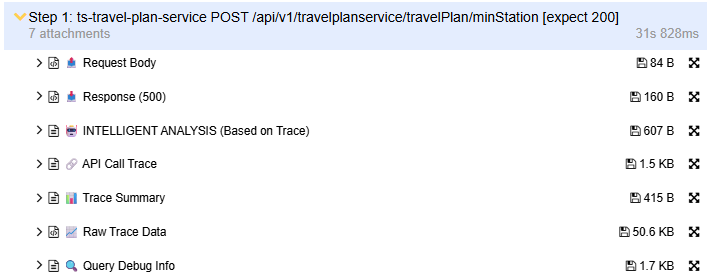
\includegraphics[width=\linewidth,trim=8 8 8 8,clip]{figs/experiment/Step_output.png}
\caption{Allure report structure for a single test step. The interface consolidates HTTP request/response data with trace-driven intelligence and includes root cause analysis alongside raw Jaeger data.}
\label{fig:step_output}
\end{figure}

Figure~\ref{fig:step_output} illustrates the comprehensive data structure captured for a single test step. When the system executes a root API call, it attaches seven distinct artifacts to the report: 
\begin{itemize}[leftmargin=*] 
\item \textbf{Request Body and Response:} The raw HTTP data for the entry-point call. 
\item \textbf{INTELLIGENT ANALYSIS:} The AI-generated diagnosis derived from the trace. 
\item \textbf{API Call Trace and Trace Summary:} Visual and statistical representations of the backend service hierarchy. 
\item \textbf{Raw Trace Data:} The complete JSON payload from the Jaeger collector. 
\item \textbf{Query Debug Info:} Metadata regarding the trace retrieval process. 
\end{itemize}

\begin{figure}[!t] 
\centering 
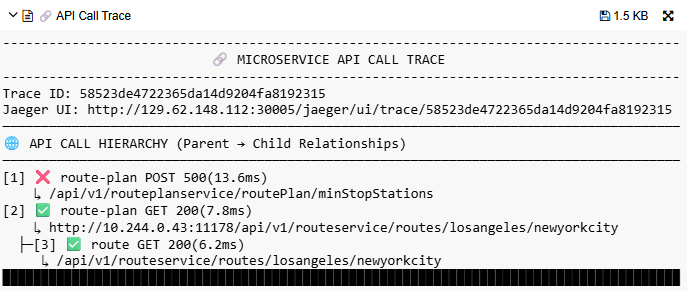
\includegraphics[width=\linewidth]{figs/experiment/api_info.png} 
\caption{Detailed API call hierarchy and performance statistics. The trace visualization reveals a POST 500 error at the root level followed by successful downstream GET calls.} 
\label{fig:api_info} 
\end{figure}tion data with backend distributed traces.

The \textit{API Call Trace} maps every internal service operation triggered by the root API and exposes the complete execution chain. Figure~\ref{fig:api_info} illustrates this hierarchy; it details an instance where a failing root request (\texttt{minStopStations}, HTTP 500) initiates interactions with successful downstream services (HTTP 200). This visualization identifies the specific failed endpoint within the internal communication flow, which facilitates rapid fault isolation. For a comprehensive diagnostic overview, the tool also provides integrated performance statistics and timing data in the \textit{Trace Summary}.

\subsection{AI-Powered Failure Diagnosis}
When the \textit{TraceErrorAnalyzer} identifies a service-level failure, it invokes the LLM-based diagnosis engine to transform raw telemetry into human-readable insights. This engine performs deep metadata inspection and correlates stack traces with span-specific context retrieved from the Jaeger trace.

\begin{figure}[!t]
    \centering
    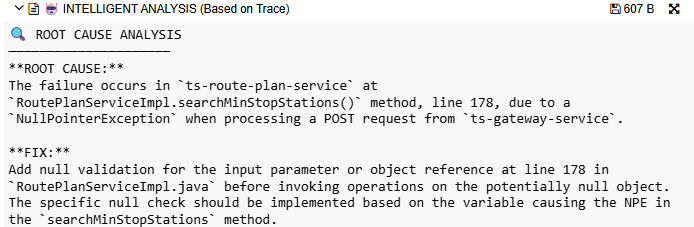
\includegraphics[width=\linewidth]{figs/experiment/INTELLIGENT_ANALYSIS.png}
    \caption{AI-generated Root Cause Analysis that identifies the failing service, method, and line number while proposing a code-level remediation.}
    \label{fig:intel_analysis}
\end{figure}

The diagnostic output, illustrated in Fig. \ref{fig:intel_analysis}, bridges the gap between high-level distributed API failures and low-level source code defects. In this experimental instance, the engine localized a \texttt{NullPointerException} within the \texttt{ts-route-plan-service}. By analyzing the execution context, the system pinpointed the specific failing method and source line responsible for the crash.

Beyond mere localization, the system generates proactive remediation strategies. In this case, the system recommends the implementation of null validation for input parameters before method invocation. This capability significantly reduces the debugging overhead for microservice developers because it provides actionable entry points for repair.

% \subsection{Discussion of Observed Behaviors} The experimental outputs demonstrate several key capabilities of the Trace-Driven Root API Mode: \begin{enumerate}[leftmargin=*] \item \textbf{Correlation Accuracy:} The system successfully links a single HTTP failure to its corresponding backend trace, even when the failure involves multiple microservices. \item \textbf{Granular Visibility:} The call hierarchy (Figure~\ref{fig:api_info}) exposes exactly which service in a chain first encountered an error, preventing "masked" failures where a root error might appear generic. \item \textbf{Actionable Intelligence:} The AI diagnosis (Figure~\ref{fig:intel_analysis}) moves beyond reporting symptoms to providing actionable code fixes. Identifying a specific line number (line 178) significantly reduces the mean time to repair (MTTR) for developers. \end{enumerate}

% These outputs confirm that by anchoring execution at the root API and analyzing the resulting traces, we capture the full complexity of microservice interactions without the overhead of manual workflow construction.

\subsection{Fault Detection Comparison}
To evaluate the fault detection effectiveness of our approach, we injected 10 targeted faults into the TrainTicket system. These faults include input validation failures, format violations, and resource constraint errors; the specific details are recorded in the injected faults specification\footnote{\url{https://github.com/miaoti/Rest/blob/inject-detection/src/main/resources/My-Example/trainticket/injectedFaults/INJECTED_FAULTS.md}}. The injections were designed to simulate common microservice defects that manifest through inter-service interactions. This design facilitates a controlled assessment of detection capabilities across different tools.

\textsc{MIST} dispatched its LLM calls through the
\texttt{io.mist.llm.LLMClient} SPI bound to a local Qwen3-Coder-30B
model~\cite{qwen2024}, deployed on an NVIDIA T1000 GPU and selected for
its superior adherence to prompt structures compared to alternatives
tested on the same hardware. While more advanced models were
considered, they exhibited inconsistent format compliance, rendering
Qwen3-Coder the most reliable option under our computational
constraints. Under \texttt{-Drandom.seed=42} the LLM temperature is
gated to zero and every prompt response passes through the
\texttt{LLMCallCache}, making the entire 25-hour run deterministic in
the sense that re-execution under the same seed produces byte-identical
generated test files. The end-to-end testing process, including trace
analysis, Trace-Shape-Oracle evaluation, and AI-driven diagnosis,
required approximately 25 hours to complete.

For comparison, we evaluated the upstream \textsc{RESTest} framework
and EvoMaster~\cite{Arcuri2020}, a search-based software testing
(SBST) tool~\cite{harman2001search} that employs evolutionary
algorithms to generate system-level test cases. To ensure experimental
fairness, EvoMaster was configured with an equivalent 25-hour search
budget, allowing sufficient evolution of test cases. This alignment
accounts for the computational demands of our local LLM inference
while providing EvoMaster ample time to optimise its search process.

The results demonstrate \textsc{MIST}'s superior performance in identifying injected faults through trace-driven generation and the Trace Shape Oracle. Table~\ref{tab:fault_comparison} summarises the detection rates.



\begin{table}[h]
\centering
\caption{Fault Detection Effectiveness Comparison}
\label{tab:fault_comparison}
\begin{tabularx}{\columnwidth}{l X c}
\toprule
\textbf{Tool} & \textbf{Testing Strategy} & \textbf{Faults Detected} \\
\midrule
\textsc{RESTest} & Static Specification Analysis & 3 / 10 \\
\textsc{EvoMaster} & Search-Based Testing (SBST) & 6 / 10 \\
\textbf{\textsc{MIST}} & \textbf{Trace-Driven Generation + Trace Shape Oracle} & \textbf{10 / 10} \\
\bottomrule
\end{tabularx}
\end{table}

\paragraph{Caveat and roadmap to a multi-SUT evaluation.}
The 10/10-versus-3/10 result above is reported on a single SUT
(TrainTicket) and against a single round of injected faults; we make no
universality claim from it.  A multi-SUT evaluation following the
positioning plan---five to seven SUTs (Sock Shop, Online Boutique,
DeathStarBench Social Network, an EvoMaster benchmark, and optionally
Spotify and LanguageTool) with 30 repetitions per (tool, SUT) pair, a
fixed 60-minute budget, AutoRestTest as the primary external baseline,
and Vargha-Delaney $A_{12}$ with Mann-Whitney $U$ for statistical
testing---is the next milestone of the project.  The ablation matrix
the multi-SUT study will populate is designed to quantify exactly what
the two new contributions buy: a \textsc{MIST} configuration with the
Trace Shape Oracle disabled and the fault taxonomy frozen at its
default eight categories is expected to perform at AutoRestTest-class
levels, and the difference between that configuration and the full
\textsc{MIST} run is the claim this paper's evaluation is set up to
defend.

\bibliographystyle{IEEEtran}
% TODO: add references.bib once experiments are finalised.
\bibliography{references}
\end{document}
